\documentclass[11pt]{article}
\usepackage[margin=1in]{geometry}
\usepackage[T1]{fontenc}
\usepackage{lmodern}
\usepackage{amsmath,amssymb,amsthm,mathtools}
\usepackage{microtype,enumitem,xcolor,tikz}
\usetikzlibrary{arrows.meta,positioning,calc,decorations.pathreplacing}
\usepackage[colorlinks=true,linkcolor=blue!45!black,citecolor=blue!45!black,urlcolor=blue!45!black]{hyperref}
\hypersetup{pdftitle={Uniform quasipolynomial-time trace reconstruction},pdfauthor={OpenAI}}
\setlength{\emergencystretch}{2em}
\setlist{itemsep=3pt,topsep=5pt}
\numberwithin{equation}{section}
\newtheorem{theorem}{Theorem}[section]
\newtheorem{proposition}[theorem]{Proposition}
\newtheorem{lemma}[theorem]{Lemma}
\newtheorem{corollary}[theorem]{Corollary}
\theoremstyle{definition}
\newtheorem{definition}[theorem]{Definition}
\theoremstyle{remark}
\newtheorem{remark}[theorem]{Remark}
\newcommand{\RR}{\mathbb R}
\newcommand{\CC}{\mathbb C}
\newcommand{\ii}{\mathrm i}
\newcommand{\EE}{\mathcal E}
\newcommand{\abs}[1]{\lvert #1\rvert}
\newcommand{\norm}[1]{\lVert #1\rVert}
\DeclareMathOperator{\re}{Re}
\title{Uniform quasipolynomial-time trace reconstruction}
\author{OpenAI}
\date{October 5, 2026}
\begin{document}
\maketitle
\begin{abstract}
We give a uniform algorithm that reconstructs every binary string from
independent deletion traces when its length and rational retention
probability are known. For each fixed retention probability, both the
number of traces and the bit complexity are quasipolynomial in the string
length. More generally, we give an explicit sample bound uniform over
all rational retention probabilities, with running time polynomial in
the sample budget and the binary input length. If the deletion probability
is at most $n^{-\varepsilon}$ for fixed $\varepsilon>0$, the sample and
running-time bounds are polynomial. Reconstruction succeeds with
probability at least $2/3$ for each input string.
\end{abstract}

\section{Introduction}
A deletion trace of a binary string is obtained by retaining each position
independently with probability $p$ and concatenating the retained bits in
order. The trace contains its length and its bits, but does not identify
their original positions. Trace reconstruction asks for the original
string from independent repetitions of this experiment. We consider the
worst case: the unknown string is arbitrary, and the recovery probability
must hold separately for each string.

Knowing that a collection of statistics distinguishes every pair of
strings gives a sample bound, but an efficient decoder needs a way to
find the unknown string. We obtain such a decoder by extending separation
to a convex family of moment arrays. The resulting tests determine one
bit at a time and can be implemented using rational arithmetic.

\subsection{The uniform guarantee}
Let $n\ge2$ be the known original length and let $p=a/b\in(0,1]$ be known,
where $a,b$ are positive integers in lowest terms. Write $L$ for the total
binary length of $a$ and $b$, and put $q=1-p$. All logarithms are natural
unless a base is displayed. Define
\begin{equation}\label{eq:budget}
 \begin{split}
 \mathsf X(n,p)&=
 \begin{cases}
  1+\dfrac{\log n}{1+\log(1/q)},&q>0,\\[3pt]
  1,&q=0,
 \end{cases}\\
 B(n,p)&=p^{-1}(\log n)\mathsf X(n,p)^2
                   (1+\log\mathsf X(n,p))^6.
 \end{split}
\end{equation}

\begin{theorem}[Uniform trace reconstruction]\label{thm:main}
There exist absolute constants $C,c\ge1$ and one randomized multitape
Turing machine $\mathcal A$ with the following property. For every
$n\ge2$, every rational $p\in(0,1]$, and every $x\in\{0,1\}^n$, given
$n,p$ in binary and access to independent ordinary deletion traces of
$x$, the machine requests at most
\[
 M_C(n,p)=\left\lceil\exp\bigl(CB(n,p)\bigr)\right\rceil
\]
traces, outputs an element of $\{0,1\}^n$, and returns $x$ with probability
at least $2/3$.

For every internal random-bit sequence and every well-formed trace
stream of strings of length at most $n$, it halts within
\[
 \bigl(n+L+M_C(n,p)\bigr)^c
\]
bit operations. This bound includes preprocessing, all parameter and
finite-precision calculations, every received trace bit and delimiter,
and the output. The only oracle operation is the external generation
of the independent deletion traces.
\end{theorem}

For fixed $p$, the budget in \eqref{eq:budget} is
$O_p((\log n)^3(1+\log\log n)^6)$ as $n\to\infty$.
Thus both resources in Theorem~\ref{thm:main} are quasipolynomial.
The theorem also controls channels whose retention probability varies
with $n$, including probabilities arbitrarily close to zero or one.
Its running-time guarantee is polynomial in the permitted sample budget.
For every fixed $\kappa>0$, the regime $q\le n^{-\kappa}$ has polynomial
sample complexity in $n$ and polynomial bit complexity in $n+L$:
indeed, $\mathsf X(n,p)\le1+1/\kappa$ and $p^{-1}$ is bounded by a
constant depending only on $\kappa$, so $B(n,p)=O_\kappa(\log n)$.

\subsection{History and relation to earlier work}
Reconstructing a sequence from corrupted copies has a broad information-theoretic
history; Levenshtein studied reconstruction under several combinatorial and
probabilistic channel models~\cite{Levenshtein2001}. Batu, Kannan, Khanna,
and McGregor formulated reconstruction from independent random deletion
traces in theoretical computer science, motivated in part by sequence
alignment~\cite{BKKM2004}. The missing positions make the problem different
from coordinatewise denoising: the same trace rank can originate at many
input positions.

For a fixed deletion probability, Holenstein, Mitzenmacher, Panigrahy, and
Wieder obtained a worst-case sample bound
$\exp(\widetilde O(\sqrt n))$~\cite{HMPW2008}. In independent papers
published at STOC 2017, De, O'Donnell, and Servedio, and Nazarov and Peres,
obtained $\exp(O(n^{1/3}))$ bounds and matching limitations for methods
using only trace means~\cite{DOS2019,NP2017}. Their complex-analytic approach
connects deletion statistics to bounded-coefficient polynomials; analytic
inequalities of Borwein and Erd\'elyi are part of the background to this
method~\cite{BE1997}. The mean-based lower bound is a restriction on that
method, not on arbitrary trace algorithms.

Chase improved the general sample upper bound to
$\exp(O(n^{1/5}\log^5n))$~\cite{Chase2021Upper}. On the lower-bound side,
Holden and Lyons proved an almost-$n^{5/4}$ bound, and Chase strengthened
it to $\Omega(n^{3/2}/\log^7n)$ for fixed deletion
probability~\cite{HoldenLyons2020,Chase2021Lower}.
Burudgunte, Valiant, and Wang subsequently proved the sample bound
\[
 \exp\bigl(p^{-7/3}(\log_2n)^{c_0}\bigr)
\]
for an absolute $c_0$, using nonlocal low-order statistics and a multiscale
propagation argument~\cite[Theorem~43]{BVW2026}. This bound is
quasipolynomial when $p^{-1}$ is polylogarithmic in $n$.
Theorem~\ref{thm:main}
builds on this strategy and provides an explicit uniform reconstruction
algorithm with the displayed bit-complexity bound.

Sample complexity and reconstruction time require different arguments.
At fixed confidence, maximum likelihood achieves worst-case reconstruction
using at most $O(n)$ times the optimal sample count, but evaluating it over
all candidate strings entails a large search~\cite[Corollary~1.1 of the
full version]{CGLSZ2024}. Burudgunte, Valiant, and Wang
explicitly distinguish testing two known strings from reconstructing an
unknown string, and leave quasipolynomial-time reconstruction open for
their approach~\cite[Section~1]{BVW2026}. The additional separation proved
here concerns every positive semidefinite moment completion of a wrong
prefix. It enables constructive feasibility tests in place of a search
over complete strings. Earlier polynomial-time results already cover
low-deletion regimes~\cite{CDLSS2021LowDeletion}.

The use of nonlocal statistics is essential to the comparison with known
barriers. Chen, De, Lee, and Servedio proved strong lower bounds for
statistical queries restricted to short \emph{consecutive} trace
blocks~\cite{CDLS2024}. Our statistics involve few ranks but may span the
whole trace, as in~\cite{BVW2026}. The generating-function identity used
to transfer them from input coordinates has antecedents in higher-order
trace reconstruction~\cite{CDLSS2021Smoothed,Chase2021Upper}.

The positive moment relaxation is a Boolean instance of the semidefinite
moment and sum-of-squares framework~\cite{Lasserre2001,Parrilo2000}.
The finite feasibility iteration is related to the classical relaxation
methods of Agmon and Motzkin--Schoenberg~\cite{Agmon1954,MotzkinSchoenberg1954}.
We prove the analytic separation and the rational implementation directly;
no external trace-reconstruction or optimization theorem is needed.


\subsection{Proof strategy and additional ingredients}
The decoder estimates products of bits at specified trace ranks; those
ranks may be far apart. It then tests a proposed prefix by asking for
moments of the remaining input bits that agree with these estimates within
a prescribed tolerance.
The moment array is constrained so that the expected squared magnitude
of every polynomial up to a prescribed degree is nonnegative. Actual
distributions give such arrays, but an arbitrary feasible array need
not come from a distribution.

The central statement separates the true input from every such array
fixing a wrong prefix. Let $d$ be the first wrong position, and write
$\Delta[P]$ for the difference between the array's value on a polynomial
$P$ and its value at the true input. Then $\Delta[X_d]=\pm1$, whereas
all differences strictly before $d$ vanish. We propagate this local
signal through progressively larger distance scales. At each stage,
the statistics are weighted sums over increasing tuples of input
positions, with exponential weights on their gaps.
We track an exponentially damped Fourier sum of the
discrepancies of these tuple statistics, indexed by the last input
position. The aim is to reduce its damping and frequency while retaining
a detectable discrepancy.

Two features make this propagation compatible with the convex
relaxation. First, positivity turns polynomial moments into inner
products. If squared norms and neighboring inner products along a
chain of $J$ vectors differ from one by at most $\xi$, then a telescoping
argument bounds the endpoint error by $O(J^2\xi)$. Applied to normalized
Fourier sums and their products, this forces a detectable product whose
total frequency is small. Pairing frequencies at prescribed differences
under a Cauchy density supplies enough pairs for this chain.

Second, a Gaussian contour deformation converts each such product back
into a tuple statistic with smaller decay and frequency. The paths joining
consecutive positions in each old tuple, together with links between their
endpoints, form a connected graph.
A spanning tree assigns distinct edges to the new gaps, controlling
the coefficient mass under interleaving. This retains the signal while
the tuple order increases by a factor of at most four.

After the last scale, a generating-function identity transfers input
statistics to ordinary trace statistics. In this identity, the channel
substitution $z=q+pw$ maps the unit disk in a trace gap parameter $w$
to the disk $|z-q|\le p$ in the corresponding input parameter $z$.
A single complex strip moves all input gap parameters into these disks
simultaneously.
This supplies the quantitative separation theorem without requiring
the algorithm to search for any of the analytic witnesses.

Finally, when the empirical estimates are sufficiently accurate, a true
prefix has a moment completion with strict slack: give
independent uniform signs a sufficiently small weight in a mixture with
its true completion. This preserves the statistical tolerance while making
the moment matrix positive definite. We exploit that
slack with an explicit sequence of rational updates, exact positivity
tests, and rounding to a fixed dyadic grid. A fixed iteration cap gives
the worst-stream bound in Theorem~\ref{thm:main}.

Section~\ref{sec:setup} introduces the relaxation.
Section~\ref{sec:multiscale} proves the multiscale step, and
Section~\ref{sec:separation} transfers its signal to traces.
Section~\ref{sec:decoding} constructs the decoder and proves
Theorem~\ref{thm:main}.

\section{Moment relaxations and prefix separation}\label{sec:setup}

We first describe the finite collection of statistics used by the decoder
and the convex set against which they will separate the true input.
Throughout, $[n]=\{1,\ldots,n\}$ and $X_1,\ldots,X_n$ are formal Boolean
variables. Products and degrees are understood after the reductions
$X_i^2=X_i$.

\subsection{Observable trace moments}
For a nonempty rank set $I=\{\ell_1<\cdots<\ell_k\}\subseteq[n]$,
the corresponding trace observable is the product of the bits at those
ranks, with value zero if the trace has length less than $\ell_k$.
Let $T_I(X)$ be its channel expectation, regarded as a polynomial in
the input bits. More explicitly,
\[
 T_I(X)=\sum_{i_1<\cdots<i_k}
    c_{I;i_1,\ldots,i_k}\,X_{i_1}\cdots X_{i_k},
\]
where $c_{I;i_1,\ldots,i_k}$ is the probability that the selected input
positions appear at ranks $\ell_1,\ldots,\ell_k$ in a deletion trace.
These events are disjoint as the input tuple varies. Consequently the
coefficients are nonnegative, their sum is at most one, and the degree
is at most $k$. They are rational when $p$ is rational. The algorithm
will estimate $T_I(x)$ by averaging the observable over independent
traces; it never observes the input positions that determine the
coefficients.

\subsection{Positive moment arrays}

The following Boolean moment relaxation is a specialization of the
semidefinite moment and sum-of-squares frameworks of
Lasserre~\cite[Section~2]{Lasserre2001} and
Parrilo~\cite[Sections~4.2--4.3]{Parrilo2000}. We use only its defining
positivity condition and elementary consequences, proved below.
Fix a proposed prefix $u\in\{0,1\}^d$ and an integer $D\ge1$.
On the remaining positions $U=\{d+1,\ldots,n\}$, use sign variables
$Y_i=2X_i-1$, so $Y_i^2=1$. A moment array consists of real numbers
$m_J$ for $J\subseteq U$ with $|J|\le2D$, including $m_\varnothing=1$,
subject to
\begin{equation}\label{eq:moment-matrix}
 \mathcal M_D(m)=
 \bigl(m_{I\triangle J}\bigr)_{
       I,J\subseteq U,\ |I|,|J|\le D}\succeq0.
\end{equation}
Only existing subsets are indexed; thus the definition also applies
when $D>|U|$ or $U$ is empty.

The array defines a functional $\EE$ on polynomials of degree at most
$2D$ by substituting $X_i=u_i$ for
$i\le d$, expanding the other bits as $(1+Y_i)/2$, reducing $Y_i^2=1$,
and setting $\EE[\prod_{i\in J}Y_i]=m_J$. We extend this functional
complex linearly. We call it a \emph{positive moment functional of order
$2D$ fixing $u$}. This terminology asserts \eqref{eq:moment-matrix},
not the existence of a probability distribution realizing all its moments.

\begin{lemma}[Elementary moment bounds]\label{lem:moment-bounds}
For every array satisfying \eqref{eq:moment-matrix}, one has
$|m_J|\le1$ for $|J|\le2D$. The value under $\EE$ of any product of at
most $2D$ distinct input bits has magnitude at most one. On polynomials
of degree at most $D$, the form
\[
 \langle P,R\rangle_{\EE}=\EE[P\overline R]
\]
is a positive semidefinite Hermitian form, linear in its first argument.
It satisfies Cauchy--Schwarz and becomes an inner product after
quotienting by its zero-norm subspace.
\end{lemma}

\begin{proof}
The empty moment equals one. Every nonempty $J$ with $|J|\le2D$ can be partitioned as $J=I\sqcup K$ with
$|I|,|K|\le D$. The $I,K$ principal submatrix in
\eqref{eq:moment-matrix} has diagonal entries one and off-diagonal
entry $m_J$, giving $|m_J|\le1$. Expanding a product of unfixed bits
as $2^{-t}\prod(1+Y_i)$ is a convex combination of these sign monomials;
fixed bits either remove factors or make the product zero. This proves
the second assertion. The final assertion is the Gram-form
interpretation of the real symmetric positive semidefinite matrix
\eqref{eq:moment-matrix}, extended to complex coefficient vectors.
Cauchy--Schwarz follows by applying positivity to $P+zR$ for $z\in\CC$;
it also shows that every zero-norm vector is orthogonal to every vector,
so the quotient is well defined.
\end{proof}

Fix a true input $x\in\{0,1\}^n$ and a prefix $u$ of length $d$ with
\[
 u_i=x_i\quad(i<d),\qquad u_d=1-x_d.
\]
For a positive moment functional fixing $u$, write
\[
 \Delta[P]=\EE[P]-P(x).
\]
Then $\Delta[X_d]=\pm1$, and $\Delta[P]=0$ whenever $P$ uses only
positions strictly before $d$. If $P$ is a linear combination of bit
monomials of degree at most $2D$, Lemma~\ref{lem:moment-bounds} gives
\begin{equation}\label{eq:delta-coefficients}
 |\Delta[P]|\le2\sum_A |c_A|
 \quad\text{when }P=\sum_A c_A\prod_{i\in A}X_i.
\end{equation}

For $p<1$, introduce
\begin{equation}\label{eq:aux-parameters}
 q_* =\max(q,1/n),\qquad
 Q=1+\log(1/q_*),\qquad
 Y=1+\frac{\log n}{Q}.
\end{equation}
When $q\ge1/n$, $Y=\mathsf X(n,p)$. When $q<1/n$,
$1\le\mathsf X(n,p)\le Y<2$. Hence
\[
 \mathsf X(n,p)\le Y\le2\mathsf X(n,p),\qquad
 QY=Q+\log n\le C\log n
\]
for an absolute constant $C$, since $n\ge2$.

\begin{theorem}[Separation from a wrong prefix]\label{thm:separation}
There exist absolute constants $C_{\mathrm{sep}}\ge1$ and an integer
$H\ge1$ with the following property. For $n\ge2$ and $0<p<1$, define
\[
 D_*=4^{\lceil\log_2 Y\rceil+H}\le4^{H+1}Y^2,
\]
using \eqref{eq:aux-parameters}. For every $x\in\{0,1\}^n$, every
$d\in[n]$, and every positive moment functional of order $2D$ fixing
$x_1,\ldots,x_{d-1},1-x_d$, where $D\ge D_*$, some nonempty
$I\subseteq[n]$ with $|I|\le D_*$ satisfies
\[
 |\EE[T_I]-T_I(x)|>
       \exp\bigl(-C_{\mathrm{sep}}B(n,p)\bigr).
\]
\end{theorem}

The theorem concerns every feasible array, including arrays not
represented by distributions. Its proof occupies the next two sections.
Once it is available, empirical trace moments rule out every wrong
extension of a correct prefix. Section~\ref{sec:decoding} shows how to
find the feasible extension with an explicit bounded computation.

\subsection{Exponentially weighted tuple statistics}
For the analytic proof, fix $x,d,\EE$ as above. For $1\le k\le2D$,
an \emph{order-$k$ feature}
is a sequence of polynomials
\begin{equation}\label{eq:feature}
 f_j=\sum_{i_1<\cdots<i_k=j}
       X_{i_1}\cdots X_{i_k}
       \prod_{h=1}^{k-1}z_h^{i_{h+1}-i_h},
 \qquad j\in[n],
\end{equation}
where $z_h=\exp(-a_h+\ii\theta_h)$, $a_h>0$, and $\theta_h\in\RR$.
For $k=1$ this means $f_j=X_j$. Put
\[
 H_f=\prod_{h=1}^{k-1}(1+1/a_h).
\]
Summing geometric series in the positive gaps shows that $H_f\ge1$
bounds the sum of the absolute coefficients of each $f_j$, since
$(1-e^{-a})^{-1}\le1+1/a$ for $a>0$.
For $s>0$ and $\omega\in\RR$, define its signal by
\begin{equation}\label{eq:signal}
 \mathcal S_f(s,\omega)=
 \sum_{j=1}^n\Delta[f_j]e^{(-s+\ii\omega)(j-d)}.
\end{equation}
Every monomial in $f_j$ uses positions at most $j$, so
$\Delta[f_j]=0$ for $j<d$. Thus, despite the centered exponent,
only nonnegative distances contribute to \eqref{eq:signal}.
The purpose of the multiscale argument is to preserve a detectable
signal while reducing $s$ and $|\omega|$, at the cost of increasing $k$.

\section{Moving a signal to a larger scale}\label{sec:multiscale}

The signal in \eqref{eq:signal} discounts positions beyond distance about
$1/s$ from the first disagreement.  The next proposition moves such a signal
to a much smaller decay parameter.  It permits an increase in feature order,
but keeps the loss in the logarithm of the signal below a factor of eight.
Controlling the angles of the new parameters is equally important: those
bounds will later permit passage from input coordinates to trace coordinates.
Enlarging spatial scales while increasing statistic order follows the
strategy of Burudgunte, Valiant, and Wang~\cite{BVW2026}.  Here the comparison
functional may be a positive truncated moment functional, and the scale step
uses Gram matrices of polynomial vectors.

\begin{proposition}[One multiscale step]\label{prop:multiscale}
There are absolute constants $0<\beta,\eta_0<1$ and $C_0,C_1\ge1$ with the
following property.  Let $f$ be an order-$k$ feature from
\eqref{eq:feature}, and let $\Delta$ arise from a moment functional of order
$2D$ with the prefix conditions of Section~\ref{sec:setup}.  Suppose
\[
 0<S\le4,\qquad 0<S'\le\min\{1,\eta_0S\},\qquad 4k\le D,
\]
and, for some $\beta S\le s\le S$ and $\abs{\omega}\le2.002s$,
\begin{equation}\label{eq:multiscale-cost}
 \abs{\mathcal S_f(s,\omega)}\ge e^{-E},\qquad
 E\ge C_0\left(1+k\log(2k)+\log H_f+\log\frac1{S'}\right).
\end{equation}
Then an order-$k'$ feature $f'$, with $1\le k'\le4k$, satisfies
\begin{equation}\label{eq:multiscale-output}
 \abs{\mathcal S_{f'}(s',\omega')}\ge e^{-7.98E},\qquad
 \beta S'\le s'\le S',\qquad \abs{\omega'}\le2.002s',
\end{equation}
and
\begin{equation}\label{eq:multiscale-height}
 H_{f'}\le H_f^4\left(1+\frac1{\beta S'}\right)^3.
\end{equation}
Moreover, there are $1\le m\le4$ lists, each equal to the old parameter list
$(z_1,\ldots,z_{k-1})$ or its complex conjugate, and at most $m-1$ added
parameters, with the following property.  Each new inner-gap parameter is a
nonempty product using at most one entry from each list and at most one added
parameter.  Every added parameter $e^{-a+\ii\theta}$ obeys
\begin{equation}\label{eq:added-parameters}
 a\ge\beta S',\qquad \abs{\theta}\le C_1S.
\end{equation}
\end{proposition}

The proof has two parts.  First, a broad Gaussian window turns the original
signal into Fourier sums.  Positivity of the moment functional then forces a
product of at most four such sums to retain a signal while its total frequency
is small.  Second, expanding that product and deforming Gaussian contours
produces a single feature with the asserted parameters.  The first part
occupies the present subsections; the conversion is carried out in
Section~\ref{subsec:contour-conversion}.

\subsection{A Gaussian window and its logarithmic bound}

Throughout the proof of Proposition~\ref{prop:multiscale}, set
\begin{equation}\label{eq:window-parameters}
 \sigma=\frac{K\sqrt E}{S'},\qquad
 W(l)=\exp\left(-\frac{l^2}{2\sigma^2}\right),\qquad b=\beta S',
\end{equation}
where $K$ is a sufficiently large absolute constant.  The constants will be
chosen in the order $K$, then $\beta$ sufficiently small, then $\eta_0$
sufficiently small, and finally $C_0$ sufficiently large.  The choices of $K$
and $\beta$ will also enforce the contour estimates below.

We use the following consequence of \eqref{eq:multiscale-cost} repeatedly.
The logarithm of any fixed product of powers of
$H_f,1+\sigma,1/S',1/b$, together with a factor
$\exp(O(k\log(2k)))$, is bounded by
\[
 C\left(1+k\log(2k)+\log H_f+\log\frac1{S'}\right)+C\log E,
\]
where $C$ depends only on constants already chosen.  Increasing $C_0$ makes
this at most any prescribed positive multiple of $E$.  Only finitely many
such estimates will be required, so a single final choice of $C_0$ suffices.

For real $t$, define the polynomial and its evaluation
\begin{equation}\label{eq:window-sums}
 A(t)=\sum_{j=1}^n f_jW(j-d)e^{\ii t(j-d)},\qquad B_x(t)=A(t)(x).
\end{equation}
The coefficient bound for $f_j$ and the Gaussian sum imply that
\begin{equation}\label{eq:window-uniform-bound}
 \abs{B_x(t)},\quad \abs{\EE[A(t)]},\quad \abs{\Delta[A(t)]}
 \le U:=C H_f(1+\sigma),
\end{equation}
with $C$ absolute and chosen so that $U\ge1$.
By prefix cancellation,
\[
 P(z):=\sum_{j=d}^n\Delta[f_j]W(j-d)z^{j-d}
 \quad\hbox{satisfies}\quad P(e^{\ii t})=\Delta[A(t)].
\]
We first show that $P$ retains a signal at almost the original decay:
\begin{equation}\label{eq:window-interior-signal}
 \abs{P(e^{-s_1+\ii\omega})}\ge\tfrac12e^{-E}
 \quad\hbox{for some}\quad \abs{s_1/s-1}\le10^{-4}.
\end{equation}

Let $V$ be a centered real normal variable with variance $\sigma^{-2}$.
Since $W(l)\mathbf E e^{Vl}=1$,
\[
 \mathcal S_f(s,\omega)=\mathbf E\,P(e^{-s+V+\ii\omega}).
\]
Write $\delta=10^{-4}$.  Exponential tilting gives
\[
 W(l)\mathbf E\big[e^{Vl}\mathbf1_{\{\abs V>\delta s\}}\big]
 =\Pr\!\left(\abs{N(l/\sigma^2,\sigma^{-2})}>\delta s\right).
\]
For $0\le l\le\delta s\sigma^2/2$, this probability is at most
$2e^{-c\delta^2s^2\sigma^2}$.  For larger $l$, use the bound one and sum
$e^{-sl}$.  Because $\abs{\Delta[f_j]}\le2H_f$, the contribution from
$\abs V>\delta s$ is at most
\begin{equation}\label{eq:window-tail}
 2H_f(1+1/s)\left(2e^{-c\delta^2s^2\sigma^2}
                      +e^{-\delta s^2\sigma^2/2}\right).
\end{equation}
Here $1/s\le1/(\beta S')$, and
$s^2\sigma^2\ge\beta^2K^2E/\eta_0^2$.  Choose $\eta_0$ sufficiently small
and then $C_0$ sufficiently large to make \eqref{eq:window-tail} less than
$e^{-2E}$.  The integral over $\abs V\le\delta s$ consequently has magnitude
at least $e^{-E}-e^{-2E}\ge e^{-E}/2$.  Its maximum integrand magnitude is
at least that large, proving \eqref{eq:window-interior-signal}.

Set
\[
 \Lambda(t)=\log\frac{U}{\abs{P(e^{\ii t})}}\ge0,
\]
with value $+\infty$ at a boundary zero.  We claim
\begin{equation}\label{eq:poisson-log-bound}
 \int_{\RR}\Lambda(t)\frac{s_1\,dt}
 {\pi(s_1^2+(t-\omega)^2)}\le1.001E.
\end{equation}
For completeness, the Cauchy Fourier transform is
\begin{equation}\label{eq:cauchy-transform}
 \int_{\RR}\frac{e^{\ii\xi v}}{\pi(1+v^2)}\,dv=e^{-\abs\xi}.
\end{equation}
For $\xi>0$, close the contour in the upper half-plane and take the residue
at $\ii$; for $\xi<0$ use the lower half-plane, and for $\xi=0$ integrate
directly.  Thus periodizing the density in
\eqref{eq:poisson-log-bound} gives the circle Poisson measure at
$e^{-s_1+\ii\omega}$.

To apply it, factor the nonzero polynomial $P$ into linear factors.  A factor
with a root outside the disk has harmonic logarithmic magnitude inside.  For
a root $a$ inside, the boundary identity
$\abs{e^{\ii t}-a}=\abs{1-\overline a e^{\ii t}}$ and the inequality
\[
 \abs{1-\overline a z}^2-\abs{z-a}^2
 =(1-\abs a^2)(1-\abs z^2)\ge0
\]
give the corresponding upper bound by its Poisson integral.  Roots on the
circle follow by a radial limit; their logarithmic singularities are
integrable.  Summing over factors yields
\[
 \int_{\RR}\Lambda(t)\frac{s_1\,dt}{\pi(s_1^2+(t-\omega)^2)}
 \le\log U-\log\abs{P(e^{-s_1+\ii\omega})}
 \le E+\log(2U).
\]
The last term is at most $1.001E$ by the choice of $C_0$, proving the claim.

\subsection{Frequencies at prescribed differences}

We seek a frequency $\lambda\in[-2s_1,2s_1]$ with a large signal and pairs
of frequencies with every prescribed difference in that interval.
The product $A(t)\overline{A(t')}$ has signed frequency $t-t'$.
After normalization by their evaluations at $x$, these products will supply
the interior vectors of a chain from $1$ to a normalized copy of
$A(\lambda)$, with consecutive frequency labels differing by at most $b$.
Each neighboring inner product will then have
signed frequency of magnitude at most $b$, even though $\abs\lambda$ may
be much larger.  The logarithmic estimate makes the required existence of
pairs a question about pairing Cauchy mass.

\begin{lemma}[Cauchy matching]\label{lem:cauchy-matching}
Let $w(v)=1/(\pi(1+v^2))$.  For every $r\ge0$ there is a finite positive
measure $\mu_r$ on $\RR^2$, supported on $v-v'=r$, such that the sum of its
two marginals is bounded above by $w(v)\,dv$.  For $r>0$ its total mass is
\begin{equation}\label{eq:cauchy-matching-mass}
 2\mu_r(\RR^2)=1-\frac4\pi\arctan(e^{-\pi/r});
\end{equation}
for $r=0$ its total mass is $1/2$.  In particular, the quantity in
\eqref{eq:cauchy-matching-mass} is greater than $0.737$ when $0<r\le2$.
\end{lemma}

\begin{proof}
For $r=0$, put half the measure $w(v)\,dv$ on the diagonal.  Suppose $r>0$,
and partition the line into chains $v+jr$, $j\in\mathbb Z$, with
$-r/2\le v<r/2$.  Abbreviate $w_j=w(v+jr)$.  On the edge from $j$ to $j-1$,
for $j\ge1$, put weight
\[
 e_j=\sum_{m\ge0}(-1)^m w_{j+m}.
\]
These weights are nonnegative, since the summands decrease along the tail.
Moreover $e_j+e_{j+1}=w_j$, so the edges exhaust the weight at every positive
vertex.  Construct the negative-side edges in the same way, proceeding from
the negative tail toward zero.  The only possibly unused weight is at the
central vertex, where its value is
\[
 R(v)=\sum_{j\in\mathbb Z}(-1)^j w(v+jr).
\]
To check that no weight has been overused, periodize $w$ at period $2r$ and
subtract its translate by $r$.  By \eqref{eq:cauchy-transform}, with
$\tau=e^{-\pi/r}$, this gives the absolutely convergent Fourier series
\[
 R(v)=\frac2r\sum_{m\ge0}\tau^{2m+1}
                  \cos\frac{(2m+1)\pi v}{r}.
\]
Writing $a=\pi v/r$, the sum equals
\[
 \re\frac{\tau e^{\ii a}}{1-\tau^2e^{2\ii a}}
 =\frac{\tau(1-\tau^2)\cos a}
        {1-2\tau^2\cos(2a)+\tau^4}\ge0,
\]
since $\abs a\le\pi/2$.  Orient every edge with its larger endpoint first
and integrate the edge weights with respect to $dv$ over $[-r/2,r/2)$.
The resulting measure has the asserted marginal domination.  Its uncovered
mass is
\[
 \int_{-r/2}^{r/2}R(v)\,dv
 =\frac4\pi\sum_{m\ge0}\frac{(-1)^m\tau^{2m+1}}{2m+1}
 =\frac4\pi\arctan\tau,
\]
which proves \eqref{eq:cauchy-matching-mass}.  The expression decreases with
$r$, and at $r=2$ it exceeds $0.737$.  For example,
$e^{-\pi/2}<0.209$ together with
$\arctan u\le u-u^3/3+u^5/5$ for $0\le u\le1$ proves this numerical bound.
\end{proof}

\begin{lemma}[Frequencies from the logarithmic bound]\label{lem:good-frequencies}
Let $s_1,E>0$, let $\abs\omega\le2.003s_1$, and let
$\Lambda:\RR\to[0,\infty]$ be measurable and satisfy
\eqref{eq:poisson-log-bound}.  There is a real $\lambda$ with
\begin{equation}\label{eq:single-frequency}
 \abs\lambda\le2s_1,\qquad \Lambda(\lambda)\le2.40E.
\end{equation}
There is also an absolute $C_2$ such that, for every $\abs y\le2s_1$, some
real $t,t'$ satisfy
\begin{equation}\label{eq:paired-frequencies}
 t-t'=y,\qquad \abs t,\abs{t'}\le C_2s_1,\qquad
 \Lambda(t)+\Lambda(t')\le2.74E.
\end{equation}
\end{lemma}

\begin{proof}
The Cauchy mass of $[-2s_1,2s_1]$ is at least
\[
 \frac{\arctan(2-2.003)+\arctan(2+2.003)}\pi>0.418.
\]
Because $1.001/0.418<2.40$, averaging proves
\eqref{eq:single-frequency}.

For \eqref{eq:paired-frequencies}, use Lemma~\ref{lem:cauchy-matching} with
$r=\abs y/s_1\le2$ and then substitute $t=\omega+s_1v$.  Reverse the
orientation if needed.  The sum of the two marginals is bounded by the
Cauchy measure in \eqref{eq:poisson-log-bound}, while twice the total pair
mass is greater than $0.737$.  Discard pairs with an endpoint outside
$[-C_2s_1,C_2s_1]$.  Twice the discarded pair mass is at most twice the
Cauchy tail outside that interval, which tends uniformly to zero as
$C_2\to\infty$, since $\abs\omega/s_1\le2.003$.
Choose an absolute $C_2$ so the retained pair mass exceeds $0.733/2$.
Its integral of $\Lambda(t)+\Lambda(t')$ is at most $1.001E$.  Some retained
pair consequently has sum at most
\[
 \frac{2(1.001)}{0.733}E<2.74E,
\]
as required.  The diagonal construction gives the same argument when $y=0$.
\end{proof}

\subsection{A product with small total frequency}

The window parameters satisfy $\abs\omega/s_1\le2.002/0.9999<2.003$, so
Lemma~\ref{lem:good-frequencies} applies to our $\Lambda$.
Individual frequencies in \eqref{eq:paired-frequencies} need not be small.
Their differences, however, can be prescribed.  We use these pairs to build
a chain of polynomial vectors whose neighboring inner products have small
total frequency.  The following Hilbert-space fact explains why such a chain
preserves the needed exponential accuracy.

\begin{lemma}[Gram chaining]\label{lem:gram-chain}
Let $v_0,\ldots,v_J$, with $J\ge1$, lie in a complex Hilbert space whose
inner product is linear in its first argument.  Suppose $\norm{v_0}=1$ and,
for some $\xi\ge0$,
\[
 \abs{\norm{v_i}^2-1}\le\xi\quad(0\le i\le J),\qquad
 \abs{\langle v_i,v_{i-1}\rangle-1}\le\xi\quad(1\le i\le J).
\]
Then
\[
 \abs{\langle v_J,v_0\rangle-1}\le2J^2\xi.
\]
\end{lemma}

\begin{proof}
Put $h_i=v_i-v_{i-1}$.  The hypotheses give
\[
 \norm{h_i}\le2\sqrt\xi,\qquad
 \abs{\langle h_i,v_{i-1}\rangle}\le2\xi,
 \qquad \norm{v_{i-1}-v_0}\le2(i-1)\sqrt\xi.
\]
Thus Cauchy--Schwarz implies
\[
 \abs{\langle h_i,v_0\rangle}
 \le2\xi+4(i-1)\xi.
\]
Sum over $i$ and use $\langle v_0,v_0\rangle=1$.
\end{proof}

Choose an absolute $C_3$ large enough that all frequencies supplied by
Lemma~\ref{lem:good-frequencies} have magnitude at most $C_3S$.
A product of one to four factors, each of the form $A(t)$ or
$\overline{A(t)}$ with $\abs t\le C_3S$, is called \emph{balanced} if the
sum of its signed frequencies has magnitude at most $b$; conjugation changes
the sign of a frequency.

\begin{lemma}[A balanced product retains a signal]\label{lem:balanced-product}
Some balanced product $G$ satisfies
\begin{equation}\label{eq:balanced-product-signal}
 \abs{\Delta[G]}\ge e^{-7.94E}.
\end{equation}
\end{lemma}

\begin{proof}
Suppose to the contrary that every balanced product has signal less than
$\epsilon=e^{-7.94E}$.  The squared modulus $\abs{A(t)}^2$ is one such
product.  Positivity of $\EE$, applied to $A(t)$ and $1$, gives
\[
 \abs{\EE[A(t)]}^2\le\EE[\abs{A(t)}^2]
 \le\abs{B_x(t)}^2+\epsilon,
\]
and hence
\begin{equation}\label{eq:evaluation-lower-bound}
 \abs{\Delta[A(t)]}\le2\abs{B_x(t)}+\sqrt\epsilon.
\end{equation}
At $\lambda$ from \eqref{eq:single-frequency}, this implies
\begin{equation}\label{eq:endpoint-normalization}
 \abs{B_x(\lambda)}\ge e^{-2.41E}.
\end{equation}
Indeed $\abs{\Delta[A(\lambda)]}\ge e^{-2.40E}$, whereas
$\sqrt\epsilon=e^{-3.97E}$; fixed numerical factors are absorbed by the
absolute lower bound on $E$ in \eqref{eq:multiscale-cost}.
For a pair in \eqref{eq:paired-frequencies}, nonnegativity of $\Lambda$
implies that both corresponding signals are at least $e^{-2.74E}$, and
\[
 \abs{\Delta[A(t)]\Delta[A(t')]}
 =U^2e^{-\Lambda(t)-\Lambda(t')}\ge e^{-2.74E}.
\]
Applying
\eqref{eq:evaluation-lower-bound} to each therefore gives
\begin{equation}\label{eq:pair-normalization}
 \abs{B_x(t)\overline{B_x(t')}}\ge e^{-2.75E}.
\end{equation}
For example, each evaluation is at least one third of its corresponding
signal once $E$ is large; the resulting factor $1/9$ is absorbed in $e^{-0.01E}$.

Take a monotone chain
$0=y_0,y_1,\ldots,y_J=\lambda$ with consecutive distances at most $b$ and
\[
 1\le J\le C(1+S/b).
\]
If $\lambda=0$, use just two endpoints and $J=1$.
For every interior $y_i$, choose a pair from
\eqref{eq:paired-frequencies} and define polynomials
\[
 V_0=1,\qquad
 V_i=\frac{A(t)\overline{A(t')}}{B_x(t)\overline{B_x(t')}}\quad(0<i<J),
 \qquad V_J=\frac{A(\lambda)}{B_x(\lambda)}.
\]
The denominators are nonzero by
\eqref{eq:endpoint-normalization}--\eqref{eq:pair-normalization}, and every
$V_i(x)$ equals one.  Regard these polynomials as vectors $v_i$ in the
Hilbert space induced by $\EE$.  They have degree at most $2k\le D$.

For $1\le i\le J$, the norm square of $v_i$ and its inner product with
$v_{i-1}$ are expectations of normalized balanced products: their signed
frequencies are respectively zero and
$y_i-y_{i-1}$, and each product has at most four factors.  The magnitude of its
normalizing denominator is at least $e^{-5.50E}$.  Our contradictory
assumption therefore gives
\[
 \abs{\norm{v_i}^2-1}\le\xi,\qquad
 \abs{\langle v_i,v_{i-1}\rangle-1}\le\xi,
 \qquad \xi=\epsilon e^{5.50E}=e^{-2.44E}.
\]
Since $v_0=1$ has norm one, Lemma~\ref{lem:gram-chain} yields
\[
 \abs{\Delta[A(\lambda)]}
 =\abs{B_x(\lambda)}\,
       \abs{\langle v_J,v_0\rangle-1}
 \le2UJ^2e^{-2.44E}<e^{-2.40E}.
\]
The final strict inequality follows by increasing $C_0$, because
$\log(2UJ^2)$ is less than $0.04E$ by \eqref{eq:multiscale-cost}.
This contradicts \eqref{eq:single-frequency} and proves the lemma.
\end{proof}

We have obtained a product of at most four windowed feature sums with signal
at least $e^{-7.94E}$ and total frequency at most $b$.  It remains to turn it
into one feature while keeping both its decay and frequency of order $S'$.
The Gaussian contour construction below supplies that final step of
Proposition~\ref{prop:multiscale}.

\subsection{Converting a balanced product to a feature}
\label{subsec:contour-conversion}

Lemma~\ref{lem:balanced-product} supplies a product of at most four windowed
Fourier sums with a substantial discrepancy and small total frequency.
We now express that product as an integral of features. The contour will
place their outer parameters in the sector required by
Proposition~\ref{prop:multiscale}; the remaining issue will be to control
the damping factors on their inner gaps.

Fix a product supplied by Lemma~\ref{lem:balanced-product}, and let
$1\le m\le4$ be its number of factors. Expand each factor in the tuples
defining $f$. An \emph{interleaving} specifies the ordering, including all
ties, of the $mk$ labeled positions in these tuples. There are at most
$(mk)^{mk}=\exp(O(k\log(2k)))$ interleavings: assigning to each labeled
position its rank among the distinct positions gives such a bound.
Only interleavings consistent with strict increase inside each old tuple
are retained. Fix one interleaving, and relabel its copies so that their
endpoints satisfy $j_1\le\cdots\le j_m$. Equal endpoints may be ordered
arbitrarily. After absorbing conjugation into the signs of the
frequencies, their window weight is
\begin{equation}
 \prod_{r=1}^m W(j_r-d)\exp\bigl(\ii t_r(j_r-d)\bigr),
 \qquad |t_r|\le C_3S,\qquad
 \left|\sum_{r=1}^m t_r\right|\le b.
 \label{eq:endpoint-window}
\end{equation}
Conjugation also conjugates the old inner-gap parameters, leaving their
dampings unchanged.

\paragraph{A Gaussian contour with controlled total frequency.}
Recall that $\sigma=K\sqrt E/S'$ and $b=\beta S'$. For every real $l$,
\begin{equation}
 W(l)=\frac{\sigma}{\ii\sqrt{2\pi}}
       \int_{-\ii\infty}^{\ii\infty}
       \exp(\sigma^2v^2/2+vl)\,dv.
 \label{eq:gaussian-contour}
\end{equation}
Indeed, writing $v=\ii u$ gives the Gaussian Fourier transform. Its value
at $l=0$ is one, and integration by parts shows that its derivative in
$l$ is $-l/\sigma^2$ times itself, proving the formula.

Set $\rho=1/2.002$. For $u=(u_1,\ldots,u_m)\in\RR^m$, define
\begin{equation}
 \Omega=\sum_{r=1}^m(u_r+t_r),\qquad
 v_r=b+\ii u_r\quad(r<m),\qquad
 v_m=-mb-\rho|\Omega|+\ii u_m.
 \label{eq:bent-contour}
\end{equation}
These real parts have partial sums $rb$ for $r<m$ and total sum
$-b-\rho|\Omega|$. When the endpoint exponent is centered at $j_m$,
the total sum gives the real part of its outer coefficient, while the
negatives of the partial sums give the real parts of the coefficients
on consecutive endpoint gaps. The contour is
therefore designed to give outer decay $b+\rho|\Omega|$ and positive
inner dampings $rb$; we verify the exact rewriting below.

For each fixed tuple of positions, first shift the first $m-1$ contours
in \eqref{eq:gaussian-contour} to their fixed vertical lines
$\re v_r=b$, leaving the last contour on the imaginary axis.
The connecting horizontal integrals vanish by Gaussian decay.
Next fix $(u_1,\ldots,u_{m-1})$ and deform the last contour to the
piecewise linear graph in \eqref{eq:bent-contour}. Its slopes have
absolute value $\rho<1$. Along horizontal segments joining its
truncations to the imaginary axis at height $\pm T$, the Gaussian
exponent has real part at most $-cT^2+O(T)$ for some $c>0$.
The factor $\exp(v_m(j_m-d))$ contributes only a linear term in $T$,
so these connecting integrals also vanish. The integrands are entire,
and hence no residues occur. This proves the identities as iterated
integrals; absolute joint convergence will follow from the next bound.

Let $\nu$ be the resulting complex measure on $\RR^m$ after the factors
depending on positions have been removed. More explicitly, outside the
measure-zero set $\Omega=0$,
\begin{equation}
 d\nu(u)=
 \left(\frac{\sigma}{\sqrt{2\pi}}\right)^m
 \exp\left(\frac{\sigma^2}{2}\sum_{r=1}^m v_r^2\right)
 \bigl(1+\ii\rho\operatorname{sgn}\Omega\bigr)\,du.
 \label{eq:contour-measure}
\end{equation}
The last factor is the differential of the bent contour divided by
$\ii\,du_m$. We next obtain estimates uniform over the frequencies in
\eqref{eq:endpoint-window}. These estimates also establish absolute
convergence of the joint integrals.

Put $\delta_0=1-4\rho^2>0$ and $c_1=\delta_0/2$. Since $m\le4$ and
$|\sum t_r|\le b$, Young's inequality gives an absolute $C_4$ such that
\begin{align}
 \sum_{r=1}^m(\re v_r)^2
 &=(m-1)b^2+(mb+\rho|\Omega|)^2 \notag\\
 &\le 3b^2+
       \left(2\rho\sqrt{\sum_r u_r^2}+(4+\rho)b\right)^2 \notag\\
 &\le (1-c_1)\sum_r u_r^2+C_4b^2.
 \label{eq:contour-quadratic}
\end{align}
The strict inequality $4\rho^2<1$ is essential here: summing at most
four imaginary coordinates can multiply their squared norm by four,
and the sector constant $2.002$ leaves a positive Gaussian decay margin.
For example,
$C_4=3+(4+\rho)^2(1+8\rho^2/\delta_0)$ suffices.
Together with \eqref{eq:contour-measure}, this proves
\[
 |d\nu(u)|\le C\sigma^m
 \exp\left(\frac{C_4\sigma^2b^2}{2}
           -\frac{c_1\sigma^2}{2}\sum_r u_r^2\right)du.
\]
For any fixed tuple of positions, the absolute value of its remaining
exponential factor is at most $\exp(C_n(1+\sum_r|u_r|))$ for a finite
constant $C_n$. This factor is integrable against the Gaussian bound.
Thus the iterated deformation also gives a jointly absolutely
convergent integral, and finite tuple sums can be interchanged with it.

Write $\mathcal U=\{u:\max_r|u_r|\le S'/16\}$. Integrating the last
bound, and splitting its negative quadratic term into two equal parts
on $\mathcal U^c$, gives absolute constants $C,C'$ with
\begin{align*}
 \|\nu\|_{\mathrm{abs}}
   &\le C\exp(C_4K^2\beta^2E/2),\\
 \int_{\mathcal U^c}|d\nu|
   &\le C'\exp\left[
      \left(\frac{C_4K^2\beta^2}{2}
                 -\frac{c_1K^2}{1024}\right)E\right].
\end{align*}
Here $\|\nu\|_{\mathrm{abs}}$ denotes total variation; the powers
$\sigma^m$ cancel under Gaussian rescaling. Choose $K$ large enough that
$c_1K^2/1024\ge30$, then choose $\beta\le1/4$ small enough that
$C_4K^2\beta^2/2\le0.001$. Increasing $C_0$ to absorb the fixed
prefactors yields
\begin{equation}
 \|\nu\|_{\mathrm{abs}}\le e^{0.005E},\qquad
 \int_{\mathcal U^c}|d\nu|\le e^{-20E}.
 \label{eq:contour-mass}
\end{equation}
This choice is consistent with the order of constants specified earlier:
$K$ is fixed first, $\beta$ second, and $\eta_0$ may then be reduced to
meet the window estimate. Only afterward is $C_0$ enlarged.

\paragraph{Outer parameters and endpoint gaps.}
For $c_r=v_r+\ii t_r$, telescoping the endpoint differences gives
\begin{equation}
 \sum_{r=1}^m c_r(j_r-d)
 =\left(\sum_{r=1}^m c_r\right)(j_m-d)
  -\sum_{r=1}^{m-1}
    \left(\sum_{l=1}^r c_l\right)(j_{r+1}-j_r).
 \label{eq:endpoint-telescoping}
\end{equation}
Consequently, the largest endpoint has coefficient
$-s'+\ii\Omega$, where
\begin{equation}
 s'=b+\rho|\Omega|.
 \label{eq:new-outer-decay}
\end{equation}
The link from $j_r$ to $j_{r+1}$ receives the parameter
\begin{equation}
 \exp\left(-rb-\ii\sum_{l=1}^r(u_l+t_l)\right),
 \qquad 1\le r<m.
 \label{eq:endpoint-link}
\end{equation}
Thus every added damping is at least $b$, for every $u$.
On $\mathcal U$,
\[
 |\Omega|\le(\beta+1/4)S',\qquad
 \beta S'\le s'\le
   \bigl[\beta+\rho(\beta+1/4)\bigr]S'\le S',
 \qquad |\Omega|\le2.002s'.
\]
The angle in \eqref{eq:endpoint-link} has absolute value at most
$3(C_3S+S'/16)\le C_1S$ for a fixed absolute $C_1$.
The outer parameters therefore satisfy the parameter inequalities in
\eqref{eq:multiscale-output}, and the endpoint links satisfy
\eqref{eq:added-parameters}. The choice of $C_1$ uses only $C_3$ and
$S'\le S$ and imposes no further condition on $K$ or $\beta$.

\subsection{Interleavings and the cost of the inner gaps}
\label{subsec:interleavings}

We have obtained outer weights at the required scale. To finish, we must
show that each interleaving has exactly the form of a feature, with
controlled coefficient sum. One old inner edge can cross several gaps
of the merged tuple, so charging its damping cost at every crossing
would overcount it. A distinct-edge assignment will prevent this loss.

For our fixed interleaving, write its distinct positions as
$i_1<\cdots<i_v$, where $1\le v\le mk$. Form a multigraph on these
vertices: include the inner edges of each old tuple and the links
between consecutive endpoints in \eqref{eq:endpoint-link}. Its edges
carry their corresponding exponential parameters. It is connected,
because each old tuple is a path to its endpoint, and the endpoint
links join those paths. Delete loops coming from equal endpoints;
their weights are one.

For each merged gap $i_{a+1}-i_a$, multiply the parameters of all edges
crossing it. Each edge length is the sum of the merged gaps it crosses,
so these new parameters reproduce the original weight exactly.
Every merged gap is crossed by some edge, by connectivity, and hence
its damping is positive. Within a single old tuple, the inner-edge
intervals have disjoint interiors. The same holds for the consecutive
endpoint links. It follows that each new parameter uses at most one
old parameter from each copy and at most one added endpoint parameter.
This is precisely the factor-count assertion in
Proposition~\ref{prop:multiscale}.

Ties merge repeated bit variables by the Boolean identity $X_i^r=X_i$
for $r\ge1$. Once the interleaving is fixed, choosing arbitrary strictly
increasing values for its $v$ distinct positions specifies exactly one
assignment to its labeled tuples. Thus no further restriction remains
on the new tuple. Its largest position is $i_v=j_m$. Summing all these
assignments gives an order-$v$ feature, denoted $f^{\mathcal I,u}$,
with outer weight $\exp((-s'+\ii\Omega)(i_v-d))$.

The following elementary fact controls its height.

\begin{lemma}[Assigning distinct edges to consecutive gaps]
\label{lem:edge-gap-assignment}
Let a connected multigraph have ordered vertices $i_1<\cdots<i_v$.
There is an assignment of a distinct edge to each gap
$(i_a,i_{a+1})$ such that its assigned edge crosses that gap.
\end{lemma}

\begin{proof}
There is nothing to prove for $v=1$. Otherwise retain a spanning tree
and orient each of its edges from its smaller to its larger endpoint.
Let $M$ be the $(v-1)\times(v-1)$ matrix whose $(e,a)$ entry is one if
tree edge $e$ crosses gap $a$, and zero otherwise. This matrix is
invertible. To see this, for an arbitrary vector $g$ in its kernel set
$y_1=0$ and $y_{a+1}=y_a+g_a$. The equation $Mg=0$ says that $y$ has
equal values at the endpoints of every tree edge. Connectivity makes
all its values zero, so $g=0$. A nonzero term in the determinant
expansion of $M$ pairs its rows and columns through entries equal to
one. That pairing is the required assignment.
\end{proof}

Figure~\ref{fig:edge-gap-assignment} shows why distinctness matters.
Although one edge may contribute to several new parameters, it need
pay for only one of their upper bounds.

\begin{figure}[htbp]
\centering
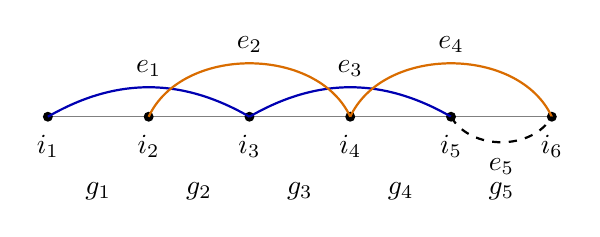
\begin{tikzpicture}[x=1.28cm,y=0.9cm,>=stealth,
  olda/.style={draw=blue!70!black,thick},
  oldb/.style={draw=orange!85!black,thick},
  added/.style={draw=black,thick,dashed}]
  \draw[gray] (0,0)--(5,0);
  \foreach \a in {1,...,6} {
    \fill (\a-1,0) circle (1.8pt);
    \node[below=3pt] at (\a-1,0) {$i_{\a}$};
  }
  \draw[olda] (0,0) to[bend left=30] node[above,pos=.5] {$e_1$} (2,0);
  \draw[olda] (2,0) to[bend left=30] node[above,pos=.5] {$e_3$} (4,0);
  \draw[oldb] (1,0) to[bend left=65] node[above,pos=.5] {$e_2$} (3,0);
  \draw[oldb] (3,0) to[bend left=65] node[above,pos=.5] {$e_4$} (5,0);
  \draw[added] (4,0) to[bend right=60] node[below=2pt,pos=.5] {$e_5$} (5,0);
  \foreach \a in {1,...,5} {
    \node at (\a-.5,-1.05) {$g_{\a}$};
  }
\end{tikzpicture}
\caption{A schematic interleaving of the two old tuples
$(i_1,i_3,i_5)$ and $(i_2,i_4,i_6)$, joined by the dashed endpoint link
$e_5$. Here $g_a$ denotes the gap $(i_a,i_{a+1})$.
The assignment $g_a\mapsto e_a$ for $1\le a\le5$ uses a distinct
crossing edge for every gap. For example,
$e_1$ crosses both $g_1$ and $g_2$, but it is charged only to $g_1$;
$e_2$ supplies the bound for $g_2$.}
\label{fig:edge-gap-assignment}
\end{figure}

Give each edge occurrence $e$ its damping $a_e>0$. The damping of a
merged gap is the sum of the $a_e$ over all edges crossing it, and is
therefore at least that of its assigned edge. Since $1+1/a$ decreases
with $a$, Lemma~\ref{lem:edge-gap-assignment} implies
\begin{align}
 H_{f^{\mathcal I,u}}
 &\le\prod_{e\text{ assigned}}(1+1/a_e)
 \le\prod_{e\text{ present}}(1+1/a_e) \notag\\
 &\le H_f^m(1+1/b)^{m-1}
 \le H_f^4(1+1/b)^3.
 \label{eq:interleaving-height}
\end{align}
The second inequality uses that all factors are at least one; the
endpoint-link dampings are $rb\ge b$. This argument includes all
overlaps between old tuples and also the case of a single distinct
position. In that case the height is the empty product one.

\paragraph{Completing the multiscale estimate.}
Apply $\Delta$ to the expanded product and use the integral
representation for each interleaving. With $\nu_{\mathcal I}$ denoting
the corresponding measure, we have the exact identity
\begin{equation}
 \Delta[\text{product}]
 =\sum_{\mathcal I}\int_{\RR^m}
   \mathcal S_{f^{\mathcal I,u}}(s',\Omega)\,d\nu_{\mathcal I}(u).
 \label{eq:product-feature-integral}
\end{equation}
All estimates above are uniform over the interleavings. The integrands
have a uniform bound even outside $\mathcal U$. Indeed, for each fixed
endpoint $j$, the coefficients of $f_j^{\mathcal I,u}$ have absolute
sum at most the height in \eqref{eq:interleaving-height}. The terms with
endpoint $j<d$ vanish under $\Delta$ by prefix agreement.
Using $s'\ge b$ gives
\begin{equation}
 \left|\mathcal S_{f^{\mathcal I,u}}(s',\Omega)\right|
 \le 2H_f^4(1+1/b)^3\sum_{l\ge0}e^{-bl}
 \le 2H_f^4(1+1/b)^4.
 \label{eq:contour-uniform-signal}
\end{equation}
In particular no exponential factor from negative distances occurs
in the tail estimate.

Let $N_{\mathrm{int}}$ be the number of interleavings and put
$V=2H_f^4(1+1/b)^4$. Hypothesis~\eqref{eq:multiscale-cost}, with a
sufficiently large absolute $C_0$, ensures
\[
 E\ge100,\qquad \log N_{\mathrm{int}}\le0.01E,
 \qquad \log V\le0.01E.
\]
Here $\log(1+1/b)$ is bounded by an absolute constant plus
$\log(1/S')$, because $b=\beta S'$, $S'\le1$, and $\beta$ has already
been fixed. If every signal in \eqref{eq:product-feature-integral}
with $u\in\mathcal U$ had magnitude below $e^{-7.98E}$, then
\eqref{eq:contour-mass} and \eqref{eq:contour-uniform-signal} would give
\[
 |\Delta[\text{product}]|
 \le N_{\mathrm{int}}
       \left(e^{(0.005-7.98)E}+Ve^{-20E}\right)
 \le e^{-7.965E}+e^{-19.98E}
 <e^{-7.94E}.
\]
This contradicts Lemma~\ref{lem:balanced-product}. Some interleaving
and some $u\in\mathcal U$ therefore give a feature with signal at least
$e^{-7.98E}$. Its order is at most $mk\le4k$;
\eqref{eq:new-outer-decay} and the bounds on $\mathcal U$ give the
required outer parameters; \eqref{eq:interleaving-height} gives
\eqref{eq:multiscale-height}; and the crossing description gives the
claimed parameter factors and \eqref{eq:added-parameters}.
This completes the proof of Proposition~\ref{prop:multiscale}.

\section{From an input signal to separation of trace moments}
\label{sec:separation}

We prove Theorem~\ref{thm:separation}.  Proposition~\ref{prop:multiscale}
preserves a detectable input-coordinate signal while reducing its decay
rate.  We first choose enough scales to make that rate at most $1/n$.
The resulting gap parameters need not belong to the disk on which trace
moments directly control the signal.  A simultaneous one-variable
continuation will bridge this difference.

Throughout this section $0<p<1$, and $q_*,Q,Y$ are as in
\eqref{eq:aux-parameters}.  Recall from Section~\ref{sec:setup} that
\begin{equation}
  1\le \mathsf X(n,p)\le Y\le 2\mathsf X(n,p),
  \qquad QY=Q+\log n\le C\log n.
  \label{eq:aux-comparisons}
\end{equation}
\subsection{A scale schedule and the surviving signal}

Set
\begin{equation}
  \mu=7.98,\qquad \alpha=0.001,\qquad
  h=\lceil\log_2Y\rceil+H,\qquad D_*=4^h,
  \label{eq:separation-cutoff}
\end{equation}
where the absolute integer $H$ will be fixed below.  In particular,
$D_*\le4^{H+1}Y^2$.  Fix an arbitrary positive moment functional of
order $2D$, where $D\ge D_*$, with first wrong position $d$,
and let $\Delta$ be its
difference from evaluation at the true word, as in Section~\ref{sec:setup}.
All constants chosen below are independent of this system, $n$, and $p$.

For an absolute constant $\eta>0$, define
\begin{equation}
 S_0=4,\qquad
 S_j=\eta q_*Y^{-\alpha}S_{j-1}
               \min\{1,D_*S_{j-1}\}\quad(1\le j\le h).
 \label{eq:scale-schedule}
\end{equation}
The linear regime of this recurrence brings $D_*S_j$ below one; its
quadratic regime then makes $S_j$ small rapidly.  Both regimes will also
be used to control the arguments of the final gap parameters.

Choose an integer $J_*$ with $\alpha J_*\ge3$, and set $H=J_*+3$.
To verify the decrease precisely, write
\[
 \vartheta=\eta q_*Y^{-\alpha},\qquad t_j=D_*S_j.
\]
Then $t_j=\vartheta t_{j-1}\min\{1,t_{j-1}\}$, so, regardless of when
the quadratic regime begins,
\[
 t_{J_*}\le \vartheta^{J_*}t_0
 \le4^{H+2}\eta^{J_*}Y^{2-\alpha J_*}\le1
\]
once $\eta$ is small enough.  Require also
\[
 \eta\le\min\{\eta_0,1/4,e^{-1}\},
\]
where $\eta_0$ is from Proposition~\ref{prop:multiscale}.
Now $\log(1/\vartheta)\ge Q$, and $t_j\le1$ for $j\ge J_*$.  Iterating
$t_j=\vartheta t_{j-1}^2$ in this range gives
\begin{equation}
 t_h\le\vartheta^{\,2^{h-J_*}-1}
       \le \exp\{-Q(2^{h-J_*}-1)\}\le n^{-1},
 \qquad S_h\le n^{-1}.
 \label{eq:terminal-scale}
\end{equation}
The last inequality follows from $2^{h-J_*}\ge8Y$ and
$Q(Y-1)=\log n$.  At every transition we also have
$0<S_j\le\min\{1,\eta_0S_{j-1}\}$, as required by the proposition.

We need an upper bound on the cost of these small scales as well.
Put $A_0=Q+\log Y$.  The recurrence implies, with
$\ell_j=\max\{0,\log(1/S_j)\}$,
\[
 \ell_j\le2\ell_{j-1}+\log(1/\vartheta),\qquad
 \ell_0=0,\qquad \log(1/\vartheta)\le C A_0.
\]
Consequently
\begin{equation}
 \log(1/S_j)\le C2^jA_0\quad(0\le j\le h).
 \label{eq:scale-cost}
\end{equation}

We can now iterate Proposition~\ref{prop:multiscale}.  Begin with the
order-one feature $f_i^{(0)}=X_i$, at decay $s_0=4$ and frequency zero.
The prefix agreement gives $\Delta[X_i]=0$ for $i<d$, whereas
$\abs{\Delta[X_d]}=1$.  Since $\abs{\Delta[X_i]}\le2$ for every $i$,
\begin{equation}
 \abs{\mathcal S_{f^{(0)}}(4,0)}
 \ge1-2\sum_{r\ge1}e^{-4r}
 =1-\frac{2}{e^4-1}>\frac12.
 \label{eq:initial-signal}
\end{equation}
Use error exponents
\begin{equation}
 E_j=C_5A_0\mu^j\quad(0\le j\le h),
 \label{eq:scale-errors}
\end{equation}
where $C_5$ is an absolute constant chosen after $H$ and $\eta$.

Here are all the induction bounds.  At stage $j$ there is a feature
$f^{(j)}$ of order $k_j\le4^j$, with
\begin{equation}
 \begin{gathered}
 \beta S_j\le s_j\le S_j,
 \qquad \abs{\omega_j}\le2.002s_j,
 \qquad \abs{\mathcal S_{f^{(j)}}(s_j,\omega_j)}\ge e^{-E_j},\\
 \log H_{f^{(j)}}\le C4^jA_0.
 \end{gathered}
 \label{eq:scale-induction}
\end{equation}
The initial case follows from \eqref{eq:initial-signal} and
$H_{f^{(0)}}=1$, on increasing $C_5$.  At the transition from $j-1$ to
$j$, the degree requirement is
\[
 4k_{j-1}\le4^j\le D_*\le D.
\]
The feature-height conclusion of the proposition and
\eqref{eq:scale-cost} give
\[
 \log H_{f^{(j)}}
 \le4\log H_{f^{(j-1)}}
       +3\log\bigl(1+1/(\beta S_j)\bigr)
 \le4\log H_{f^{(j-1)}}+C2^jA_0.
\]
Summing this recurrence proves the last bound in
\eqref{eq:scale-induction}.  To check the exponent hypothesis of the
proposition, its bracket at this transition is at most
\[
 C\bigl(1+j4^{j-1}+4^{j-1}A_0+2^jA_0\bigr).
\]
Because $\mu>4$, the sequences
$j(4/\mu)^{j-1}$ and $2^j/\mu^{j-1}$ are bounded.  Thus one fixed
choice of $C_5$ makes this bracket times $C_0$ at most $E_{j-1}$ for
every $j$.  All hypotheses of Proposition~\ref{prop:multiscale} hold,
and its signal bound is $e^{-\mu E_{j-1}}=e^{-E_j}$.

Write $f=f^{(h)}$, $k=k_h$, $s=s_h$, and $\omega=\omega_h$.
We have obtained a signal of magnitude at least $e^{-E_h}$ with
$k\le D_*$ and $s\le1/n$.  The next step records where its parameters
lie in the unit disk; this information will control the cost of
continuing the signal to the trace domain.

\subsection{Damping under multiplication}

Call the parameters introduced between endpoints in each application of
Proposition~\ref{prop:multiscale} \emph{elementary parameters}.  Include
also the final outer parameter
\[
 z_0=e^{-s+\ii\omega}.
\]
An elementary parameter $e^{-a+\ii\theta}$ introduced at stage $j$
satisfies $a\ge\beta S_j$ and $\abs{\theta}\le C_1S_{j-1}$.
Using \eqref{eq:scale-schedule}, choose a sufficiently small absolute
$c_2>0$ so that all these parameters obey
\begin{equation}
 a\ge\gamma\min\{\abs{\theta},D_*\theta^2\},
 \qquad \gamma=c_2q_*Y^{-\alpha}\le1.
 \label{eq:elementary-damping}
\end{equation}
For an explicit verification, the increasing function
$u\mapsto u\min\{1,D_*u\}$ changes by at most a factor
$\max\{C_1,C_1^2\}$ when $u$ is replaced by $C_1u$.
It therefore suffices to take
$c_2\le\beta\eta/\max\{C_1,C_1^2\}$.
Shrinking $c_2$ further covers $z_0$, since
$\abs{\omega}\le2.002s$.  Conjugating any elementary parameter
preserves \eqref{eq:elementary-damping}.

Each new inner gap contains at most one parameter from each of at most
four copies of the preceding feature, and at most one new elementary
parameter.  Count repeated factors with multiplicity; conjugation does
not change the count.  Starting with no inner parameters, the maximum
number $N_j$ of elementary factors in a stage-$j$ inner gap satisfies
\[
 N_0=0,\qquad N_j\le4N_{j-1}+1,
 \qquad N_j\le\frac{4^j-1}{3}.
\]
In particular, an inner gap of $f$, even after multiplication by $z_0$,
contains at most $(4^h+2)/3\le D_*$ elementary factors.

The following elementary lemma explains why this count matters.  The
Cayley map $z\mapsto(1+z)/(1-z)$ sends the unit disk to the right
half-plane; we need a quantitative distance from its boundary.

\begin{lemma}[Products with controlled damping]
\label{lem:product-cayley}
Let $N\ge1$ be an integer and $0<\gamma\le1$.  Suppose $z$ is a
nonempty product of at most $N$ numbers $e^{-a_j+\ii\theta_j}$, where
$a_j>0$, $\theta_j\in\RR$, and
\[
 a_j\ge\gamma\min\{\abs{\theta_j},N\theta_j^2\}.
\]
There is an absolute $c_3>0$ such that
\[
 \re\frac{1+z}{1-z}\ge c_3\gamma.
\]
\end{lemma}

\begin{proof}
Write $z=e^{-T+\ii\psi}$, where $T=\sum_j a_j>0$ and
$\psi=\sum_j\theta_j$.  Let
\[
 U=\sum_{\abs{\theta_j}\ge1/N}\abs{\theta_j},
 \qquad V=\sum_{\abs{\theta_j}<1/N}\abs{\theta_j}.
\]
Summing the hypotheses and applying Cauchy--Schwarz to at most $N$
small angles yields
\[
 T\ge\gamma\left(U+N\sum_{\abs{\theta_j}<1/N}\theta_j^2\right)
   \ge\gamma(U+V^2).
\]
If $U\ge1$ or $V\ge1$, the last bracket is at least one.
Otherwise $U+V^2\ge U^2+V^2\ge(U+V)^2/2$.
Since $\abs{\psi}\le U+V$, in all cases
\[
 T\ge\tfrac12\gamma\min\{1,\psi^2\}.
\]
For $0<T\le1$ it follows that
\[
 1-\abs z^2\ge cT,\qquad
 \abs{1-z}^2\le C\bigl(T^2+\min\{1,\psi^2\}\bigr)
                 \le C'T/\gamma.
\]
Their ratio is $\re((1+z)/(1-z))$.  If $T>1$, that ratio is at least
$(1-e^{-2})/4$, which also suffices because $\gamma\le1$.
\end{proof}

\subsection{The exact trace generating identity}

Let $z_1,\ldots,z_{k-1}$ denote the inner gap parameters of the final
feature $f$.  Define the polynomial in $k$ complex variables
\begin{equation}
 F(Z_0,\ldots,Z_{k-1})
 =\sum_{1\le i_1<\cdots<i_k\le n}
  \Delta\left[\prod_{r=1}^kX_{i_r}\right]
  Z_0^{i_1}\prod_{r=1}^{k-1}Z_r^{i_{r+1}-i_r}.
 \label{eq:input-polynomial}
\end{equation}
At the point
\[
 Z_0^*=z_0,\qquad Z_r^*=z_rz_0\quad(1\le r<k),
\]
the exponents of $z_0$ telescope to $i_k$, so
\begin{equation}
 F(Z^*)=z_0^d\mathcal S_f(s,\omega),
 \qquad \abs{F(Z^*)}\ge e^{-E_h-1}.
 \label{eq:input-polynomial-signal}
\end{equation}
Here $sd\le nS_h\le1$.  Each coordinate of $Z^*$ is a nonempty
product of at most $D_*$ elementary parameters, and hence
Lemma~\ref{lem:product-cayley} gives
\begin{equation}
 \re\frac{1+Z_r^*}{1-Z_r^*}\ge c_3\gamma\quad(0\le r<k).
 \label{eq:input-cayley-margin}
\end{equation}
We shall also need a bound on the coordinates' collective proximity to
the unit circle.  If $z_r=e^{-a_r+\ii\theta_r}$, then
\[
 \frac1{1-\abs{Z_r^*}}
 \le1+\frac1{a_r+s}\le1+\frac1{a_r}\quad(r\ge1),
 \qquad
 \frac1{1-\abs{Z_0^*}}\le1+\frac1s.
\]
These inequalities follow from $e^u\ge1+u$ for $u>0$.
The height bound in \eqref{eq:scale-induction} and
\eqref{eq:scale-cost} therefore imply
\begin{equation}
 W_*:=\log\prod_{r=0}^{k-1}\frac1{1-\abs{Z_r^*}}
 \le\log H_f+\log\bigl(1+1/(\beta S_h)\bigr)
 \le C4^h A_0.
 \label{eq:input-boundary-cost}
\end{equation}

We next express the same polynomial in terms of observable trace
moments on a different domain.  This uses the multivariate trace
generating identity of~\cite[Section~5.2]{CDLSS2021Smoothed}; see also
\cite[Fact~20]{CDLS2024}.  We give the required counting argument
directly.  For a rank tuple
$\ell=(\ell_1,\ldots,\ell_k)$ with
$1\le\ell_1<\cdots<\ell_k\le n$, abbreviate
$T_\ell=T_{\{\ell_1,\ldots,\ell_k\}}$.
For $u=(u_0,\ldots,u_{k-1})\in\CC^k$, set
\[
 G(u)=\sum_{1\le\ell_1<\cdots<\ell_k\le n}
       \Delta[T_\ell]\,
       u_0^{\ell_1-1}
       \prod_{r=1}^{k-1}u_r^{\ell_{r+1}-\ell_r-1}.
\]
Then, with $Z_r=q+pu_r$, the exact polynomial identity is
\begin{equation}
 \left(\prod_{r=0}^{k-1}Z_r\right)G(u)=p^kF(Z).
 \label{eq:trace-generating-identity}
\end{equation}
To prove it, fix input positions $i_1<\cdots<i_k$ that supply the
specified retained bits.  Their own retention contributes $p^k$.
Every input position before $i_1$ contributes $q+pu_0$, according to
whether it is deleted or retained; there are $i_1-1$ such positions.
Similarly, the $i_{r+1}-i_r-1$ positions in the $r$th intervening gap
each contribute $q+pu_r$.  Positions after $i_k$ contribute a total
factor of one.  The retained counts in these intervals are exactly
$\ell_1-1$ and $\ell_{r+1}-\ell_r-1$.  Summing over all input tuples
and applying $\Delta$ gives $G(u)$ as $p^k$ times the polynomial in
\eqref{eq:input-polynomial} with every displayed gap exponent reduced
by one.  Multiplication by $\prod_rZ_r$ proves
\eqref{eq:trace-generating-identity}, including points where some
$Z_r=0$.

Suppose, for the moment, that
\begin{equation}
 \abs{\Delta[T_I]}\le\varepsilon
 \quad\text{for every }I\subseteq\{1,\ldots,n\}
 \text{ with }1\le\abs I\le D_*,
 \label{eq:trace-closeness}
\end{equation}
where $\varepsilon>0$.  Since $k\le D_*$, the rank sum has at most
$n^k$ terms, so $\abs{G(u)}\le n^k\varepsilon$ when all
$\abs{u_r}\le1$.  On this polydisk $\abs{Z_r}\le q+p=1$.
Thus \eqref{eq:trace-generating-identity} gives
\begin{equation}
 \abs{F(Z)}\le (n/p)^k\varepsilon
 \qquad\text{if }\abs{Z_r-q}\le p\quad(0\le r<k).
 \label{eq:trace-polydisk-bound}
\end{equation}
This calculation uses only ordinary trace ranks and the convention that
a rank product is zero when the trace is too short.

\subsection{Simultaneous continuation and the separation bound}

The lower bound \eqref{eq:input-polynomial-signal} and the upper bound
\eqref{eq:trace-polydisk-bound} concern different points.  In Cayley
coordinates the disk $\abs{Z-q}\le p$ becomes a half-plane:
\begin{equation}
 \abs{Z-q}\le p
 \quad\Longleftrightarrow\quad
 \re\frac{1+Z}{1-Z}\ge\frac qp
 \qquad(\abs Z<1).
 \label{eq:cayley-trace-disk}
\end{equation}
Indeed, writing $w=(1+Z)/(1-Z)$ and expanding
$\abs{pw-(1+q)}^2\le p^2\abs{w+1}^2$ reduces it to
$4q\le4p\re w$.  We will move all coordinates to this half-plane
using one complex variable.  A single strip interpolation avoids
incurring a separate continuation loss for every coordinate.

Write
\[
 w_r=\frac{1+Z_r^*}{1-Z_r^*}=\xi_r+\ii\zeta_r,
 \qquad \xi_r\ge c_3\gamma,
\]
where $\xi_r,\zeta_r\in\RR$.  For $v\in\CC$ set
\begin{equation}
 w_r(v)=(1+v)\xi_r+\ii\zeta_r,
 \qquad Z_r(v)=\frac{w_r(v)-1}{w_r(v)+1},
 \qquad
 R=1+\frac{q}{pc_3\gamma}.
 \label{eq:simultaneous-path}
\end{equation}
Figure~\ref{fig:simultaneous-cayley} shows how a common real value of
$v$ moves two possible starting coordinates into the trace half-plane.
The proof uses the analytic maps \eqref{eq:simultaneous-path} for complex
$v$ throughout a strip.

\suppressfloats[t]
\begin{figure}[htbp]
\centering
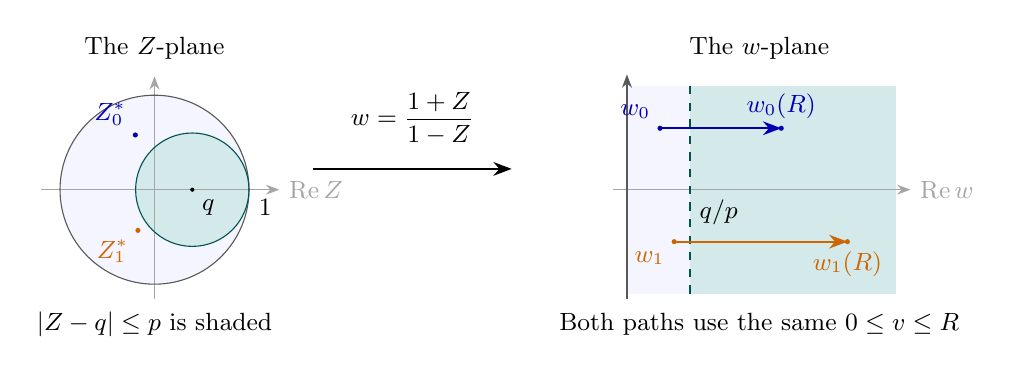
\begin{tikzpicture}[x=1.2cm,y=1.2cm,>=Stealth,font=\small]
 \begin{scope}
  \fill[blue!4] (0,0) circle (1);
  \fill[teal!17] (0.4,0) circle (0.6);
  \draw[black!35,->] (-1.2,0)--(1.32,0) node[right] {$\re Z$};
  \draw[black!35,->] (0,-1.16)--(0,1.2);
  \draw[black!65] (0,0) circle (1);
  \draw[teal!65!black] (0.4,0) circle (0.6);
  \fill (0.4,0) circle (0.022) node[below right] {$q$};
  \node[below right] at (1,0) {$1$};
  \fill[blue!70!black] (-0.2027,0.5791) circle (0.027)
       node[above left] {$Z_0^*$};
  \fill[orange!80!black] (-0.1753,-0.4310) circle (0.027)
       node[below left] {$Z_1^*$};
  \node at (0,1.5) {The $Z$-plane};
  \node at (0,-1.42) {$\abs{Z-q}\le p$ is shaded};
 \end{scope}
 \draw[->,thick] (1.68,0.22)--(3.78,0.22)
       node[midway,above=5pt] {$w=\dfrac{1+Z}{1-Z}$};
 \begin{scope}[xshift=6cm]
  \fill[blue!4] (0,-1.1) rectangle (2.85,1.1);
  \fill[teal!17] (0.6667,-1.1) rectangle (2.85,1.1);
  \draw[black!35,->] (-0.15,0)--(3,0) node[right] {$\re w$};
  \draw[black!65,->] (0,-1.16)--(0,1.22);
  \draw[dashed,teal!65!black] (0.6667,-1.1)--(0.6667,1.1);
  \node[below right] at (0.6667,0) {$q/p$};
  \draw[->,thick,blue!70!black] (0.35,0.65)--(1.6333,0.65);
  \fill[blue!70!black] (0.35,0.65) circle (0.027)
        node[above left] {$w_0$};
  \fill[blue!70!black] (1.6333,0.65) circle (0.027)
        node[above] {$w_0(R)$};
  \draw[->,thick,orange!80!black] (0.5,-0.55)--(2.3333,-0.55);
  \fill[orange!80!black] (0.5,-0.55) circle (0.027)
        node[below left] {$w_1$};
  \fill[orange!80!black] (2.3333,-0.55) circle (0.027)
        node[below] {$w_1(R)$};
  \node at (1.4,1.5) {The $w$-plane};
  \node at (1.4,-1.42) {Both paths use the same $0\le v\le R$};
 \end{scope}
\end{tikzpicture}
\caption{Schematic geometry of the simultaneous continuation.
The Cayley map turns the deletion disk into
$\re w\ge q/p$.  Two possible starting coordinates are shown.
The horizontal arrows have different lengths but share the same
parameter: $w_r(v)=(1+v)\re w_r+\ii\operatorname{Im}w_r$.
Only their real traces $0\le v\le R$ are drawn.  The proof interpolates
$F(Z_0(v),\ldots,Z_{k-1}(v))$ on a single complex strip, simultaneously
for every coordinate.}
\label{fig:simultaneous-cayley}
\end{figure}

On the closed strip $-1/2\le\re v\le R$ we have
$\re w_r(v)=(1+\re v)\xi_r>0$, so all $Z_r(v)$ lie in the unit
disk and depend analytically on $v$.  At $v=0$ they equal $Z_r^*$.
On the right boundary,
\[
 \re w_r(v)=(1+R)\xi_r\ge q/p,
\]
and therefore \eqref{eq:trace-polydisk-bound} applies.  Moreover
\begin{equation}
 1+R\le C\frac{Y^\alpha}{p},
 \label{eq:strip-width}
\end{equation}
because $\gamma=c_2q_*Y^{-\alpha}$ and $q\le q_*$.

We need a bound on the left boundary that does not involve $n^k$.
The identity $1-\abs{Z}^2=4\re w/\abs{w+1}^2$ gives, when
$\re v=-1/2$,
\begin{equation}
 1-\abs{Z_r(v)}
 \ge\frac{1-\abs{Z_r^*}}{4(1+\abs v)^2}.
 \label{eq:left-boundary-distance}
\end{equation}
To check the constant, first use
$1-\abs{Z_r(v)}\ge \xi_r/\abs{w_r(v)+1}^2$ and
$1-\abs{Z_r^*}\le4\xi_r/\abs{w_r+1}^2$.
Then use
\[
 \abs{w_r(v)+1}\le\abs{w_r+1}+\xi_r\abs v
                   \le(1+\abs v)\abs{w_r+1}.
\]
The coefficients of $F$ have magnitude at most two.  Summing
independent geometric series over the positive prefix and gap lengths
therefore gives, for every point in the open unit polydisk,
\[
 \abs{F(Z)}\le2\prod_{r=0}^{k-1}\frac1{1-\abs{Z_r}}.
\]
It follows from \eqref{eq:left-boundary-distance} that
\[
 g(v):=\frac{F(Z_0(v),\ldots,Z_{k-1}(v))}{(2+v)^{2k}}
\]
has the boundary bounds
\begin{equation}
 \begin{aligned}
 \log\abs{g(v)}&\le W_*+Ck+C
                    &&(\re v=-1/2),\\
 \log\abs{g(v)}&\le k\log(n/p)+\log\varepsilon
                    &&(\re v=R).
 \end{aligned}
 \label{eq:strip-side-bounds}
\end{equation}
On the left, $(1+\abs v)/\abs{2+v}$ is bounded by an absolute
constant.  On the right, $\abs{2+v}\ge2+R>1$.
The function $g$ is analytic and bounded on the strip: $F$ is a finite
polynomial evaluated in the unit polydisk, and $\abs{2+v}\ge3/2$.

For clarity, the strip estimate we use is the following elementary
consequence of the maximum principle.  If a bounded analytic function
on $a\le\re v\le b$ has logarithmic boundary bounds $L_-,L_+$,
then at a real $t\in[a,b]$ its logarithm is at most
$((b-t)L_-+(t-a)L_+)/(b-a)$.  Multiply the function by the exponential
of the negative affine interpolant to make both side bounds one.
On rectangles of height tending to infinity, apply the maximum
principle after multiplying further by
$\exp\{\tau(v^2-\max\{a^2,b^2\})\}$, for $\tau>0$.
This factor has modulus at most one on the vertical sides and tends
uniformly to zero on the horizontal sides.  Let the height tend to
infinity and then $\tau$ tend to zero.  This proves the estimate,
including zeros of the function by continuity.

At $t=0$ in our strip, the right boundary has weight $1/(2R+1)$.
By \eqref{eq:input-polynomial-signal},
$\log\abs{g(0)}\ge-E_h-1-2k\log2$.
Substituting \eqref{eq:strip-side-bounds} consequently gives
\begin{align}
 \log(1/\varepsilon)
 &\le k\log(n/p)+(2R+1)(E_h+1+2k\log2)
             +2R(W_*+Ck+C)\notag\\
 &\le k\log(n/p)
       +C(1+R)\bigl(E_h+4^hA_0\bigr).
 \label{eq:separation-exponent}
\end{align}
This is the desired quantitative transfer from input coordinates to
trace coordinates.

It remains to compare the exponent with the budget in
\eqref{eq:budget}.  Put $t=\log_2\mu$.  The choices in
\eqref{eq:separation-cutoff} satisfy $t+\alpha<3$, and
\[
 4^h\le CY^2,\qquad E_h\le CA_0Y^t,
 \qquad A_0\le Q(1+\log Y),\qquad QY\le C\log n.
\]
Thus \eqref{eq:strip-width} yields
\begin{align*}
 (1+R)E_h
 &\le \frac Cp(\log n)Y^{t+\alpha-1}(1+\log Y)
 \le \frac Cp(\log n)Y^2(1+\log Y),\\
 (1+R)4^hA_0
 &\le \frac Cp(\log n)Y^{1+\alpha}(1+\log Y)
 \le \frac Cp(\log n)Y^2(1+\log Y).
\end{align*}
Also, since $n\ge2$ and $\log(1/p)\le1/p$,
\[
 k\log(n/p)\le CY^2\bigl(\log n+\log(1/p)\bigr)
                \le \frac Cp(\log n)Y^2.
\]
Using \eqref{eq:aux-comparisons}, we conclude that the right-hand side
of \eqref{eq:separation-exponent} is at most
\begin{equation}
 \frac Cp(\log n)Y^2(1+\log Y)
 \le C_6 p^{-1}(\log n)\mathsf X(n,p)^2
                  (1+\log\mathsf X(n,p))^6
 =C_6B(n,p).
 \label{eq:final-B-bound}
\end{equation}
Taking $\varepsilon=e^{-C_{\mathrm{sep}}B(n,p)}$ with
$C_{\mathrm{sep}}>C_6$ contradicts
\eqref{eq:separation-exponent}.  Hence
\eqref{eq:trace-closeness} fails for that $\varepsilon$, proving
Theorem~\ref{thm:separation} with the cutoff
\eqref{eq:separation-cutoff}.

All constants were fixed in the following order: those of
Proposition~\ref{prop:multiscale}; then $J_*,H$ and $\eta$; then
$C_5,c_2$; and finally $C_{\mathrm{sep}}$.  There is no dependence on
the denominator of $p$ or on how close it is to an endpoint.
In particular, when $q<1/n$ the cutoff $q_*=1/n$ keeps $Y<2$ and
$Q=1+\log n$, while $q/q_*\le1$ keeps the strip estimate uniform.
When $p$ is small, the strip width is controlled by the single factor
$p^{-1}$ already present in the budget.  The case $p=1$ will be handled
directly in the decoding argument.

\section{A uniform decoder}\label{sec:decoding}

Theorem~\ref{thm:separation} supplies a test for the first incorrect bit of
a prefix: no moment system fixing that prefix can reproduce all the
low-order trace statistics.  To turn this statement into an algorithm,
we must also recognize a correct prefix in bounded time.  The useful
additional fact is that a correct prefix admits a moment system with
strict slack, both in its statistical constraints and in its positivity
constraint.  We first exhibit that slack, then give a rational procedure
which is guaranteed to find a feasible system whenever such slack exists.

\subsection{Statistical constraints for a prefix}

Assume for now that \(p<1\).  Choose an integer \(D\) and a positive dyadic
number \(\zeta=2^{-b_\zeta}\) such that
\begin{equation}\label{eq:decoder-parameters}
 D_*\le D\le C Y^2,\qquad
 \zeta\le \tfrac14,\qquad
 4\zeta<e^{-C_{\mathrm{sep}}B(n,p)},\qquad b_\zeta=O(B(n,p)),
\end{equation}
where \(C_{\mathrm{sep}}\) is the constant in
Theorem~\ref{thm:separation}.  Integer formulas for these choices will be
given below.  Let
\[
 \mathcal I_D=\{I\subseteq\{1,\ldots,n\}:1\le |I|\le D\},
 \qquad N=|\mathcal I_D|,
 \qquad T=512(1+N)\zeta^{-2}.
\]
The number \(T\) is an integer.  From \(T\) independent traces, form the
empirical mean \(\widehat t_I\) of the rank observable defining \(T_I\),
for every \(I\in\mathcal I_D\).  These are observables of the ordinary
trace: if a requested rank is absent, its observable is zero.

For each fixed input \(x\), let \(\mathcal G\) be the event
\begin{equation}\label{eq:empirical-good}
 |\widehat t_I-T_I(x)|\le \zeta/8
 \quad\text{for every }I\in\mathcal I_D.
\end{equation}
Each observable takes values in \(\{0,1\}\), so its empirical mean has
variance at most \(1/(4T)\).  Chebyshev's inequality and a union bound give
\begin{equation}\label{eq:good-probability}
 \mathbb P_x(\mathcal G^c)
 \le \frac{16N}{T\zeta^2}\le\frac1{32}.
\end{equation}
The same event will control all the prefix tests, even though the
prefixes are chosen using the data.

For a proposed prefix, use the remaining sign variables and their moment
matrix \(M(m)=\mathcal M_D(m)\) from \eqref{eq:moment-matrix}.  Its nonempty moment
coordinates form a real vector \(m\).  Consider the rational constraints
\begin{equation}\label{eq:prefix-feasibility}
 m\in[-1,1]^l,\qquad M(m)\succeq0,\qquad
 |\EE_m[T_I]-\widehat t_I|\le\zeta
 \quad(I\in\mathcal I_D),
\end{equation}
where \(l\) is the number of moment coordinates.  Substituting the prefix
and writing each remaining bit as one half of one plus its sign makes
\(\EE_m[T_I]\) an affine function of \(m\).  Its nonconstant coefficients
have absolute sum at most \(1\), by the coefficient bound for \(T_I\)
in Section~\ref{sec:setup}.

\begin{lemma}\label{lem:prefix-slack}
On \(\mathcal G\), a prefix whose first incorrect bit is at its last
position has no solution to \eqref{eq:prefix-feasibility}.  Every correct
prefix has a moment vector \(m^*\in[-1,1]^l\) such that, writing \(G\)
for the dimension of its moment matrix,
\begin{equation}\label{eq:prefix-slack}
 M(m^*)\succeq(\zeta/8)\operatorname{Id}_G,\qquad
 |\EE_{m^*}[T_I]-\widehat t_I|\le\zeta/2
 \quad(I\in\mathcal I_D).
\end{equation}
\end{lemma}

\begin{proof}
If a wrong prefix had a feasible moment vector, then
\eqref{eq:empirical-good} and \eqref{eq:prefix-feasibility} would give
\[
 |\EE_m[T_I]-T_I(x)|\le 9\zeta/8
 \quad(I\in\mathcal I_D).
\]
This contradicts Theorem~\ref{thm:separation} and
\eqref{eq:decoder-parameters}.

For a correct prefix, take the moments of the true completion with
weight \(1-\zeta/8\), and the moments of independent uniform signs on
the remaining positions with weight \(\zeta/8\).  The moment matrix of
the latter distribution is the identity: its \((I,J)\) entry is zero
unless \(I=J\).  The mixture therefore has the stated matrix lower
bound, and its coordinates lie in \([-1,1]\).  Both constituent
distributions give channel expectations in \([0,1]\), so mixing changes
each \(T_I(x)\) by at most \(\zeta/8\).  Equation~\eqref{eq:empirical-good}
then bounds the discrepancy from \(\widehat t_I\) by \(\zeta/4\),
which is stronger than required.
\end{proof}

\subsection{Finding a moment system with slack}

The next lemma gives the bounded procedure needed for
\eqref{eq:prefix-feasibility}.  It only promises to succeed when there
is slack; every reported solution satisfies the exact inequalities.
This distinction avoids any need to decide arbitrary instances of
semidefinite feasibility.
The procedure is a projected relaxation method for inequalities, in
the tradition of Agmon and Motzkin--Schoenberg
\cite{Agmon1954,MotzkinSchoenberg1954}.  We give the iteration and its
rounding analysis explicitly.

\begin{lemma}[Rational feasibility with slack]\label{lem:rational-feasibility}
Let \(r\ge0\) and \(D\ge1\) be integers, and let \(m\) consist of the
\[
 l=\sum_{j=1}^{\min(2D,r)}\binom rj
\]
nonempty sign moments.  Let \(M(m)\) be their moment matrix, of
dimension
\[
 G=\sum_{j=0}^{\min(D,r)}\binom rj.
\]
Suppose a finite list of rational affine inequalities
\(\ell_t(m)\le b_t\) is given, each with nonconstant coefficient vector
of \(\ell^1\)-norm at most \(1\), together with a dyadic
\(0<\zeta\le1/4\).

There is a deterministic rational procedure which either returns a
vector satisfying
\[
 m\in[-1,1]^l,\qquad M(m)\succeq0,\qquad \ell_t(m)\le b_t
 \quad\text{for all }t,
\]
or reports failure.  It returns a vector whenever some
\(m^*\in[-1,1]^l\) satisfies
\[
 M(m^*)\succeq(\zeta/8)\operatorname{Id}_G,\qquad
 \ell_t(m^*)\le b_t-\zeta/2\quad\text{for all }t.
\]
Put \(\lambda=\zeta/(16G)\).  The procedure performs at most
\(\lceil10(1+l)/\lambda^2\rceil\) feasibility checks, each taking a
number of bit operations polynomial in the list dimensions, the
input bit lengths, and \(\log(1/\zeta)\).  These time bounds hold
without the slack assumption.
\end{lemma}

\begin{proof}
If \(l=0\), the matrix is \([1]\) and all inequalities are constant,
so direct rational comparisons suffice.  Suppose \(l>0\).  We describe
exact separating directions, then an iteration with bounded precision.

\paragraph{Directions from violated constraints.}
At a current point \(m^{\mathrm{cur}}\in[-1,1]^l\), first check the
affine inequalities and the matrix condition exactly.  If all hold,
return the current vector.  A violated inequality
\(\ell_t(m^{\mathrm{cur}})>b_t\) gives the direction \(a\) equal to
minus its nonconstant coefficient vector.  Then \(\norm{a}_2\le1\);
under the slack assumption,
\[
 \langle m^*-m^{\mathrm{cur}},a\rangle\ge\zeta/2\ge\lambda.
\]

If instead the matrix condition fails, find a nonzero rational vector
\(v\) with \(v^\top M(m^{\mathrm{cur}})v<0\).  The exact construction
of \(v\) is given just below.  Write the associated affine form as
\[
 v^\top M(m)v=c+h\cdot m,\qquad
 a=\frac{h}{Gv^\top v}.
\]
Each matrix entry is either the constant \(1\) or one moment
coordinate.  Consequently
\[
 \norm{h}_1\le\norm{v}_1^2\le G\norm{v}_2^2,
 \qquad \norm{a}_2\le1.
\]
The slack matrix lower bound gives
\[
 \langle m^*-m^{\mathrm{cur}},a\rangle
 =\frac{v^\top(M(m^*)-M(m^{\mathrm{cur}}))v}{Gv^\top v}
 \ge\frac{\zeta}{8G}\ge\lambda.
\]
Thus either violated condition provides a rational direction satisfying
\begin{equation}\label{eq:feasibility-direction}
 \norm{a}_2\le1,\qquad
 \langle m^*-m^{\mathrm{cur}},a\rangle\ge\lambda
\end{equation}
whenever a slack solution exists.  If a constant affine inequality is
violated, its direction is zero; this cannot happen in the slack case,
and in all other cases the iteration is still bounded.

\paragraph{An exact matrix check.}
For a rational symmetric matrix, eliminate a positive diagonal pivot
by taking its Schur complement.  Congruence by an invertible triangular
matrix shows that the original matrix is positive semidefinite exactly
when the positive pivot and this Schur complement are.  A negative
diagonal supplies a negative unit vector.  If a remaining diagonal at
\(i\) is zero and its entry \(b\) in column \(j\) is nonzero, let \(c\)
be the diagonal at \(j\).  We may assume \(c\ge0\), since otherwise
there is already a negative diagonal.  The rational vector
\[
 y=e_i-\frac{b}{1+c+|b|}e_j
\]
has quadratic form
\[
 \frac{b^2}{(1+c+|b|)^2}
 \bigl[-2(1+c+|b|)+c\bigr]<0.
\]
If no negative vector is found, continue with a positive diagonal
pivot; when none remain, all entries are zero and the remainder is
positive semidefinite.

For completeness, a negative vector of a Schur complement lifts to
one of the original matrix using only rational arithmetic.  If \(P\)
is the original block of eliminated pivots and \(B\) its block of
entries against the remaining indices, the lift of \(y\) is
\[
 v=(-P^{-1}By,y).
\]
Its quadratic form is exactly the quadratic form of \(y\) for the
Schur complement.

These operations have polynomial bit complexity.  Indeed, clear
denominators in a rational matrix with \(t\)-bit entries; even the
product of all denominators has at most \(G^2t\) bits.  If \(H\) is
the resulting integer matrix and its entries have at most \(s\) bits,
the determinant expansion bounds every \(j\)-row minor by
\(j!\,2^{js}\).  Its bit length is therefore \(O(G(s+\log G))\).
Schur-complement entries are ratios of minors of the original matrix,
and the inverse formula for \(P\) gives the same bound for the lift.
Fraction-reduced elimination, with rational comparisons at each step,
therefore computes the check and the negative vector in polynomially
many bit operations.  This argument applies however small a positive
pivot or a negative quadratic form may be.

\paragraph{Iteration and rounding.}
Start with \(m^{\mathrm{cur}}=0\).  Choose the dyadic grid with mesh
\[
 \eta=2^{-g},\qquad
 g=\left\lceil\log_2\frac{100(1+l)}{\lambda^2}\right\rceil.
\]
The integer \(g\) is computed by rational comparisons with powers of
two; thus \(\eta\le\lambda^2/(100(1+l))\), with
\(O(1+\log((1+l)/\lambda))\) fractional bits.  After an
unsuccessful check, add \(\lambda a\), clip every coordinate to
\([-1,1]\), and round to the nearest point of this grid in the box.
The endpoints of the box belong to the grid.  Repeat up to the
stated number of checks, reporting failure if none accepts.

Under the slack assumption, \eqref{eq:feasibility-direction} implies
\[
 \norm{m^{\mathrm{cur}}+\lambda a-m^*}_2^2
 \le \norm{m^{\mathrm{cur}}-m^*}_2^2-\lambda^2.
\]
Clipping cannot increase the distance to \(m^*\).  Since both the
clipped vector and \(m^*\) lie in the box, rounding changes the squared
distance by at most \(4l\eta+l\eta^2<\lambda^2/2\).  Each failed check
thus decreases squared distance by at least \(\lambda^2/2\).
Its initial value is at most \(l\), so acceptance must occur before
the cap.

Finally, rounding keeps every iterate on a single grid of the indicated
bit length.  The exact matrix check, the affine comparisons, the
formation and normalization of \(h\), and one update involve
polynomially many rational operations on numbers of polynomial bit
length.  Temporary denominators within an update therefore have
polynomial bit length, and they do not accumulate across updates.
The fixed cap and these bounds apply to every rational input list,
whether or not it admits a slack solution.
\end{proof}

For a prefix test, write each absolute-value constraint in
\eqref{eq:prefix-feasibility} as two affine inequalities and apply
Lemma~\ref{lem:rational-feasibility}.  Lemma~\ref{lem:prefix-slack}
verifies exactly the slack hypotheses for a correct prefix.  Every
acceptance, on any data, gives an actual moment system satisfying
\eqref{eq:prefix-feasibility}.

The decoder starts with the empty prefix and tests both one-bit
extensions.  If precisely one accepts, it appends that bit; otherwise
it appends \(0\).  It repeats until the prefix has length \(n\).
The latter rule specifies a length-\(n\) output even for data on which
the statistical estimates fail.  There are at most \(2n\) tests.

\subsection{Integer parameters and bit complexity}

We now make the choices in \eqref{eq:decoder-parameters} using only
the binary input.  This also accounts for the size of every list and
every rational calculation in the decoder.  Continue to assume
\(p<1\), and use \(q_*,Q,Y\) from \eqref{eq:aux-parameters}.  Define
the positive integers
\begin{align*}
 u&=1+\lceil\log_2 n\rceil,
 &v&=1+\lfloor\log_2(1/q_*)\rfloor,\\
 y&=1+\lceil u/v\rceil,
 &w&=1+\lceil\log_2 y\rceil,
 &a_p&=\lceil1/p\rceil.
\end{align*}
All logarithms appearing in these integer formulas mean integer
length comparisons.  In particular, the integer part of a logarithm
of a rational number is found by comparing its numerator with
power-of-two multiples of its denominator.  The rational maximum
defining \(q_*\) is also found by an integer comparison.

The elementary comparisons
\[
 u\asymp\log n,\qquad v\asymp Q,\qquad
 Y\le y\le C Y,\qquad
 w\asymp1+\log Y,\qquad p^{-1}\le a_p\le2p^{-1}
\]
have absolute constants.  For the asserted lower bound on \(y\),
use \(u\ge(\log n)/\log2\) and \(v\le Q/\log2\).
Together with \(Y\asymp\mathsf X(n,p)\), these comparisons give
\begin{equation}\label{eq:integer-budget-proxy}
 B(n,p)\le a_pu y^2w^6\le C B(n,p).
\end{equation}
Choose fixed positive integers \(K_D,K_m\), sufficiently large for
the constants in Theorem~\ref{thm:separation}, and set
\begin{equation}\label{eq:integer-decoder-parameters}
 D=K_Dy^2,\qquad b_\zeta=K_m a_pu y^2w^6,\qquad
 \zeta=2^{-b_\zeta}.
\end{equation}
Since \(D_*\le C Y^2\) and \(B(n,p)\ge\log2\), these choices ensure
all of \eqref{eq:decoder-parameters}.  The integers \(D,b_\zeta\), in binary,
are computable in time polynomial in the input bit lengths.  Writing
the denominator \(2^{b_\zeta}\) subsequently costs \(O(b_\zeta)\) bits, which will
be included in the bounds below.

We next describe how to form the rational constraints.  For
\(I=\{l_1<\cdots<l_k\}\) and \(i_1<\cdots<i_k\), the coefficient
of \(X_{i_1}\cdots X_{i_k}\) in \(T_I\) is
\begin{equation}\label{eq:explicit-channel-coefficient}
 \binom{i_1-1}{l_1-1}
 \prod_{j=1}^{k-1}
 \binom{i_{j+1}-i_j-1}{l_{j+1}-l_j-1}
 \,p^{l_k}q^{i_k-l_k},
\end{equation}
when all the gap counts are possible, and is zero otherwise.
Indeed, the selected positions must be retained, and the prefix and
successive open gaps must contain the indicated numbers of additional
retentions.  Positions after \(i_k\) are unrestricted.  Formula
\eqref{eq:explicit-channel-coefficient} follows by multiplying these
independent binomial probabilities.

If the input representation is \(p=a/b\), every denominator in
\eqref{eq:explicit-channel-coefficient} divides \(b^n\).
Binomial coefficients have \(O(n)\) bits.  Sign expansion adds a
denominator dividing \(2^D\), and empirical means have denominator
\(T\).  Consequently the constraint coefficients have polynomial
bit length in \(n+L+D+\log T\).  Enumerating the rank and input tuples,
then expanding the resulting bit monomials and substituting the
prefix, constructs them directly.  No list of complete trace masks
is required.

All these enumerations fit the permitted resource scale.  From
\(D=O(Y^2)\), \(Y\asymp\mathsf X(n,p)\), and \eqref{eq:budget},
\begin{equation}\label{eq:decoder-size-bound}
 D\log n=O(B(n,p)).
\end{equation}
The rank list, every matrix basis, and every moment list have size
at most \((n+1)^{2D}=\exp(O(B(n,p)))\).  Input tuple lists satisfy the
same bound.  A sign expansion has at most \(2^D\) terms; products
of these enumeration bounds remain \(\exp(O(B(n,p)))\).  Subsets
larger than the available number of positions are simply absent,
so this statement includes \(D>n\) and prefixes with very few
remaining positions.

By \eqref{eq:decoder-parameters}, the trace count \(T\) is
\(\exp(O(B(n,p)))\).  For every prefix, the iteration cap in
Lemma~\ref{lem:rational-feasibility} is bounded by
\[
 2560(1+l)G^2\zeta^{-2}+1=\exp(O(B(n,p))).
\]
The bit length of its grid is
\(O(b_\zeta+\log G+\log(1+l))=O(B(n,p))\).
The preceding coefficient bounds and that lemma therefore bound
all computation by a fixed polynomial in
\begin{equation}\label{eq:decoder-total-resource}
 n+L+\exp(O(B(n,p))).
\end{equation}
In particular, this includes the construction of parameters and
constraints, exact rational arithmetic, and the at most \(2n\)
prefix tests.

\begin{proof}[Proof of Theorem~\ref{thm:main}]
If \(p=1\), request one trace and output it.  For the universal
halting specification, output \(0^n\) if the supplied well-formed
trace has a different length.  The actual channel always supplies
the input itself, and this branch takes polynomially many bit
operations in \(n+L\).

For \(p<1\), use \eqref{eq:integer-decoder-parameters}, request the
specified \(T\) traces, and compute their empirical statistics.
Run the prefix rule specified above.  This defines the machine on
every stream of well-formed traces.

On \(\mathcal G\), induction on the prefix length shows that
precisely the correct extension accepts: the incorrect extension
is infeasible by Lemma~\ref{lem:prefix-slack}, and the correct one
has the slack that guarantees acceptance.  Thus the output is \(x\)
on \(\mathcal G\), whose probability is at least \(31/32>2/3\) for
each fixed \(x\).

Each supplied trace has at most \(n\) bits and one delimiter.
Reading them, and computing each of the finitely many rank
observables, costs polynomially many bit operations in \(n+T+N\);
the empirical counters have \(O(\log T)\) bits.  All loops, including
all feasibility tests, have the input-dependent caps already given.
Thus \eqref{eq:decoder-total-resource} is a bound for every
well-formed trace stream, independently of the success event.
The machine can ignore its internal random bits.

To be explicit about the computational model, the described finite
lists may be stored sequentially on tapes; replacing an indexed
lookup by a scan incurs at most a polynomial overhead in their
total encoded length.  Integer addition, multiplication, division,
and fraction reduction have elementary polynomial-time multitape
implementations.  The bit-length and loop bounds above therefore
give absolute constants \(K,d\) for which the trace count is at most
\(\exp(KB(n,p))\) and the total bit cost is at most
\((n+L+\exp(KB(n,p)))^d\), after enlarging \(K,d\) to absorb fixed
factors.  This enlargement is uniform because \(B(n,p)\ge\log2\).
Choose absolute \(C,c\) large enough, with \(C\ge K\) and \(c\ge d\).
Both the sample bound \(M_C(n,p)\) and the required runtime
\((n+L+M_C(n,p))^c\) follow.  All constants used in parameter
selection are fixed integers in a single finite program.
\end{proof}

\begin{thebibliography}{99}

\bibitem{Agmon1954}
Shmuel Agmon.
The relaxation method for linear inequalities.
\emph{Canadian Journal of Mathematics} \textbf{6} (1954), 382--392.
\href{https://doi.org/10.4153/CJM-1954-037-2}{doi:10.4153/CJM-1954-037-2}.

\bibitem{BKKM2004}
Tu\u{g}kan Batu, Sampath Kannan, Sanjeev Khanna, and Andrew McGregor.
Reconstructing strings from random traces.
In \emph{Proceedings of the Fifteenth Annual ACM--SIAM Symposium on
Discrete Algorithms (SODA)}, 2004, pp.~910--918.

\bibitem{BE1997}
Peter Borwein and Tam\'as Erd\'elyi.
Littlewood-type problems on subarcs of the unit circle.
\emph{Indiana University Mathematics Journal} \textbf{46}(4) (1997),
1323--1346.
\href{https://doi.org/10.1512/iumj.1997.46.1435}{doi:10.1512/iumj.1997.46.1435}.

\bibitem{BVW2026}
Arnav Burudgunte, Paul Valiant, and Hongao Wang.
Quasipolynomial trace reconstruction.
Preprint, 2026.
\href{https://arxiv.org/abs/2607.04073v1}{arXiv:2607.04073v1}.

\bibitem{Chase2021Lower}
Zachary Chase.
New lower bounds for trace reconstruction.
\emph{Annales de l'Institut Henri Poincar\'e, Probabilit\'es et Statistiques}
\textbf{57}(2) (2021), 627--643.
\href{https://doi.org/10.1214/20-AIHP1089}{doi:10.1214/20-AIHP1089}.

\bibitem{Chase2021Upper}
Zachary Chase.
Separating words and trace reconstruction.
In \emph{Proceedings of the 53rd Annual ACM SIGACT Symposium on Theory
of Computing (STOC)}, 2021, pp.~21--31.
\href{https://doi.org/10.1145/3406325.3451118}{doi:10.1145/3406325.3451118}.
Trace-reconstruction preprint: \emph{New upper bounds for trace
reconstruction},
\href{https://arxiv.org/abs/2009.03296v3}{arXiv:2009.03296v3},
2022 (first posted 2020).

\bibitem{CDLS2024}
Xi Chen, Anindya De, Chin Ho Lee, and Rocco A.~Servedio.
Trace reconstruction from local statistical queries.
In \emph{Approximation, Randomization, and Combinatorial Optimization.
Algorithms and Techniques (APPROX/RANDOM 2024)},
LIPIcs \textbf{317} (2024), 52:1--52:24.
\href{https://doi.org/10.4230/LIPIcs.APPROX/RANDOM.2024.52}{doi:10.4230/LIPIcs.APPROX/RANDOM.2024.52}.

\bibitem{CDLSS2021LowDeletion}
Xi Chen, Anindya De, Chin Ho Lee, Rocco A.~Servedio, and Sandip Sinha.
Polynomial-time trace reconstruction in the low deletion rate regime.
In \emph{12th Innovations in Theoretical Computer Science Conference
(ITCS 2021)}, LIPIcs \textbf{185} (2021), 20:1--20:20.
\href{https://doi.org/10.4230/LIPIcs.ITCS.2021.20}{doi:10.4230/LIPIcs.ITCS.2021.20}.

\bibitem{CDLSS2021Smoothed}
Xi Chen, Anindya De, Chin Ho Lee, Rocco A.~Servedio, and Sandip Sinha.
Polynomial-time trace reconstruction in the smoothed complexity model.
In \emph{Proceedings of the 2021 ACM--SIAM Symposium on Discrete
Algorithms (SODA)}, 2021, pp.~54--73.
\href{https://doi.org/10.1137/1.9781611976465.5}{doi:10.1137/1.9781611976465.5}.
Full version: \href{https://arxiv.org/abs/2008.12386}{arXiv:2008.12386}.

\bibitem{CGLSZ2024}
Kuan Cheng, Elena Grigorescu, Xin Li, Madhu Sudan, and Minshen Zhu.
On $k$-mer-based and maximum likelihood estimation algorithms for trace
reconstruction.
In \emph{2024 IEEE International Symposium on Information Theory
(ISIT)}, 2024, pp.~879--884.
Full version: \href{https://arxiv.org/abs/2308.14993v2}{arXiv:2308.14993v2}.

\bibitem{DOS2019}
Anindya De, Ryan O'Donnell, and Rocco A.~Servedio.
Optimal mean-based algorithms for trace reconstruction.
\emph{Annals of Applied Probability} \textbf{29}(2) (2019), 851--874.
\href{https://doi.org/10.1214/18-AAP1394}{doi:10.1214/18-AAP1394}.
Conference version in STOC 2017, pp.~1047--1056.

\bibitem{HoldenLyons2020}
Nina Holden and Russell Lyons.
Lower bounds for trace reconstruction.
\emph{Annals of Applied Probability} \textbf{30}(2) (2020), 503--525.
\href{https://doi.org/10.1214/19-AAP1506}{doi:10.1214/19-AAP1506}.

\bibitem{HMPW2008}
Thomas Holenstein, Michael Mitzenmacher, Rina Panigrahy, and Udi Wieder.
Trace reconstruction with constant deletion probability and related
results.
In \emph{Proceedings of the Nineteenth Annual ACM--SIAM Symposium on
Discrete Algorithms (SODA)}, 2008, pp.~389--398.
\href{https://doi.org/10.1145/1347082.1347125}{doi:10.1145/1347082.1347125}.

\bibitem{Lasserre2001}
Jean B.~Lasserre.
Global optimization with polynomials and the problem of moments.
\emph{SIAM Journal on Optimization} \textbf{11}(3) (2001), 796--817.
\href{https://doi.org/10.1137/S1052623400366802}{doi:10.1137/S1052623400366802}.

\bibitem{Levenshtein2001}
Vladimir I.~Levenshtein.
Efficient reconstruction of sequences.
\emph{IEEE Transactions on Information Theory} \textbf{47}(1) (2001),
2--22.
\href{https://doi.org/10.1109/18.904499}{doi:10.1109/18.904499}.

\bibitem{MotzkinSchoenberg1954}
Theodore S.~Motzkin and Isaac J.~Schoenberg.
The relaxation method for linear inequalities.
\emph{Canadian Journal of Mathematics} \textbf{6} (1954), 393--404.
\href{https://doi.org/10.4153/CJM-1954-038-x}{doi:10.4153/CJM-1954-038-x}.

\bibitem{NP2017}
Fedor Nazarov and Yuval Peres.
Trace reconstruction with $\exp(O(n^{1/3}))$ samples.
In \emph{Proceedings of the 49th Annual ACM SIGACT Symposium on Theory
of Computing (STOC)}, 2017, pp.~1042--1046.
\href{https://doi.org/10.1145/3055399.3055494}{doi:10.1145/3055399.3055494}.

\bibitem{Parrilo2000}
Pablo A.~Parrilo.
\emph{Structured semidefinite programs and semialgebraic geometry
methods in robustness and optimization}.
Ph.D. thesis, California Institute of Technology, 2000.
\href{https://doi.org/10.7907/2K6Y-CH43}{doi:10.7907/2K6Y-CH43}.

\end{thebibliography}

\end{document}
